\documentclass{beamer}
\usepackage{amsmath}
\usepackage{bm}
\usepackage{amsfonts}
\usepackage{amssymb}
\usepackage{epsfig}

%\usepackage{beamerthemeJuanLesPins}  % quite good
%\usepackage{ beamerthemeMadrid}   % reasonable
%\usepackage{beamerthemeRochester} % very good, rectugularized
%\usepackage{beamerthemeSingapore} % very smooth and gives good space
%\usepackage{beamerthemeWarsaw} % excellent only the bottom problematic 
%\usepackage{}

%%%%%%%%%%%%%%%%%%%%%%%%%%%%%%%%%%%%%%%%%%%%%%%%%%%%%%%%%%%%%%%%%%%%
%
%  Utilities for typesetting in latex
%
%  Chris Williams, 1997, modified from utils.tex belonging to
%  Chris Bishop, 4 June 1995.
%
%
%%%%%%%%%%%%%%%%%%%%%%%%%%%%%%%%%%%%%%%%%%%%%%%%%%%%%%%%%%%%%%%%%%%%

\newcommand{\be}{\begin{equation}}
\newcommand{\ee}{\end{equation}}
\newcommand{\bi}{\begin{itemize}}
\newcommand{\ei}{\end{itemize}}
\newcommand{\bea}{\begin{eqnarray}}
\newcommand{\eea}{\end{eqnarray}}
\newcommand{\HOME}{/user/cs_neural/willicki}
%\newcommand{\COREL}{/user/cs_neural/bishopc/corel}

\newcommand{\bfdelta}{\boldsymbol{\delta}}
\newcommand{\bfDelta}{\boldsymbol{\Delta}}
\newcommand{\bfbeta}{\boldsymbol{\beta}}
\newcommand{\bfgamma}{\boldsymbol{\gamma}}
\newcommand{\bfmu}{\bm{\mu}}
%\newcommand{\bfmu}{\boldsymbol{\mu}}
\newcommand{\bfnu}{\boldsymbol{\nu}}
\newcommand{\bfalpha}{\boldsymbol{\alpha}}
\newcommand{\bfepsilon}{\boldsymbol{\epsilon}}
\newcommand{\bfSigma}{\boldsymbol{\Sigma}}
\newcommand{\bftau}{\boldsymbol{\tau}}
\newcommand{\bflambda}{\boldsymbol{\lambda}}
\newcommand{\bfLambda}{\boldsymbol{\Lambda}}
\newcommand{\bfpsi}{\boldsymbol{\psi}}
\newcommand{\bfxi}{\boldsymbol{\xi}}
\newcommand{\bfpi}{\bm{\pi}}
%\newcommand{\bfpi}{\boldsymbol{\pi}}
\newcommand{\bfPsi}{\boldsymbol{\Psi}}
\newcommand{\bfphi}{\boldsymbol{\phi}}
\newcommand{\bfPhi}{\boldsymbol{\Phi}}
\newcommand{\bfrho}{\boldsymbol{\rho}}
\newcommand{\bftheta}{\boldsymbol{\theta}}
\newcommand{\bfTheta}{\boldsymbol{\Theta}}
\newcommand{\bfomega}{\boldsymbol{\omega}}

\newcommand{\Bmath}[1]{\boldsymbol{#1}}

\newcommand{\bfa}{\mathbf{a}}
\newcommand{\bfb}{\mathbf{b}}
\newcommand{\bfc}{\mathbf{c}}
\newcommand{\bfd}{\mathbf{d}}
\newcommand{\bfe}{\mathbf{e}}
\newcommand{\bff}{\mathbf{f}}
\newcommand{\bfg}{\mathbf{g}}
\newcommand{\bfh}{\mathbf{h}}
\newcommand{\bfk}{\mathbf{k}}
\newcommand{\bfl}{\mathbf{l}}
\newcommand{\bfm}{\mathbf{m}}
\newcommand{\bfn}{\mathbf{n}}
\newcommand{\bfo}{\mathbf{o}}
\newcommand{\bfp}{\mathbf{p}}
\newcommand{\bfq}{\mathbf{q}}
\newcommand{\bfr}{\mathbf{r}}
\newcommand{\bfs}{\mathbf{s}}
\newcommand{\bft}{\mathbf{t}}
\newcommand{\bfu}{\mathbf{u}}
\newcommand{\bfv}{\mathbf{v}}
\newcommand{\bfw}{\mathbf{w}}
\newcommand{\bfx}{\mathbf{x}}
\newcommand{\bfy}{\mathbf{y}}
\newcommand{\bfz}{\mathbf{z}}

\newcommand{\bfzero}{\mathbf{0}}
\newcommand{\bfone}{\mathbf{1}}

\newcommand{\bfA}{\mathbf{A}}
\newcommand{\bfB}{\mathbf{B}}
\newcommand{\bfC}{\mathbf{C}}
\newcommand{\bfD}{\mathbf{D}}
\newcommand{\bfE}{\mathbf{E}}
\newcommand{\bfG}{\mathbf{G}}
\newcommand{\bfH}{\mathbf{H}}
\newcommand{\bfI}{\mathbf{I}}
\newcommand{\bfK}{\mathbf{K}}
\newcommand{\bfL}{\mathbf{L}}
\newcommand{\bfM}{\mathbf{M}}
\newcommand{\bfO}{\mathbf{O}}
\newcommand{\bfP}{\mathbf{P}}
\newcommand{\bfQ}{\mathbf{Q}}
\newcommand{\bfR}{\mathbf{R}}
\newcommand{\bfS}{\mathbf{S}}
\newcommand{\bfT}{\mathbf{T}}
\newcommand{\bfU}{\mathbf{U}}
\newcommand{\bfV}{\mathbf{V}}
\newcommand{\bfW}{\mathbf{W}}
\newcommand{\bfX}{\mathbf{X}}
\newcommand{\bfY}{\mathbf{Y}}
\newcommand{\bfZ}{\mathbf{Z}}
\newcommand{\llangle}{{\langle \vspace{-2mm} \langle}}
\newcommand{\rrangle}{{\rangle \vspace{-2mm} \rangle}}
\newcommand{\la}{\leftarrow}

\newcommand{\tf}{\tilde{f}}
\newcommand{\tg}{\tilde{g}}
\newcommand{\tX}{\tilde{X}}
\newcommand{\tY}{\tilde{Y}}
\newcommand{\tZ}{\tilde{Z}}

\newcommand{\bbE}{\mathbb{E}}
\newcommand{\bbR}{\mathbb{R}}
\newcommand{\bbP}{\mathbb{P}}
\newcommand{\bbT}{\mathbb{T}}
\newcommand{\bbZ}{\mathbb{Z}}

% for Fourier analysis
\newcommand{\ois}{2 \pi i s}  % ois is mnemonic for omega i of s
\newcommand{\oik}{2 \pi i k}  % ois is mnemonic for omega i of k
\newcommand{\oin}{2 \pi i n}  % ois is mnemonic for omega i of n
\newcommand{\oim}{2 \pi i m}  % ois is mnemonic for omega i of m

%\newcommand{\T}{\mathop{\rm T}\nolimits}
\newcommand{\T}{{\rm T}}
%\newcommand{\iint}{\int \! \! \int}
%\newcommand{\iiint}{\int \! \! \int \! \! \int}
\newcommand{\Tr}{\mbox{Tr}}
\newcommand{\diff}[1]{{\,d#1}}
\newcommand{\vgraph}[1]{
  \newpage
  \begin{center}
  {\large \bf #1}
  \end{center}
  \vspace{2mm}
}
%%\newcommand{\lapproxeq}{\stackrel{\textstyle <}{\sim}}
\newcommand{\high}[1]{\textcolor{blue}{\emph{#1}}}
\newcommand{\cut}[1]{}
\newcommand{\citeasnoun}[1]{\citeN{#1}}
\newcommand{\citemulti}[2]{(#1, \citeyearNP{#2})}
\newcommand{\citemultiN}[2]{#1 (\citeyearNP{#2})}
\newcommand{\Sum}{{\displaystyle \sum}}
\newcommand{\defeq}{{\stackrel{def}{=}}}
\newcommand{\marg}[1]{\marginpar{#1}}

%%%%%%%%%%%%%%%%%%%%%%%%%%%%%%%%%%%%%%%%%%%%%%%%%%%%%%%%%%%%%%%%%%%%

\newcommand{\pdt}[2]{\frac{\partial^2 #1}{\partial {#2}^2 }}
\newcommand{\pdsd}[3]{\frac{\partial^2 #1}{\partial {#2} \partial {#3} }}
\newcommand{\pdo}[2]{\frac{\partial {#1}}{\partial {#2}}}
\newcommand{\pdol}[2]{\partial {#1}/ \partial {#2}}
\newcommand{\pdu}[1]{\frac{\partial }{\partial {#1}}}                          

%%% Local Variables: 
%%% mode: latex
%%% TeX-master: t
%%% End: 


\title{Gaussian Process Modelling of Transcription 
Factor Networks using Markov Chain Monte Carlo}

\author{Michalis K. Titsias, Neil Lawrence and Magnus Rattray\\ 
School of Computer Science\\
University of Manchester}
\date{26th March 2008}


\begin{document}

\frame{\titlepage}


%\section[Outline]{}
%\frame{\tableofcontents}

\frame
{
\frametitle{Outline}

\begin{itemize}
  \item A sampling algorithm for Gaussian Process Models 
     
       %\begin{itemize}

        % \item Demonstration in 1-D regression

       %\end{itemize}

  \item Transcription Factor protein inference 
 
  \item Conclusions       

  \end{itemize}

}

%\section{Introduction}
%\subsection{Overview of the Beamer Class}
\frame
{

\frametitle{Gaussian Processes }

\begin{itemize}
\item A Gaussian process (GP) is a distribution 
            over real-valued functions
            \textcolor{red}{$f(\bfx)$}. It is defined by 
\begin{itemize} 
\item a mean function

 $$\mu(\bfx) =  E(f(\bfx))$$  

\item and a covariance or kernel function 


$$k(\bfx_n,\bfx_m) =  E(f(\bfx_n) f(\bfx_m))$$

E.g. this can be the RBF (or squared exponential) kernel

$$
k(\bfx_n,\bfx_m) = \alpha \exp\left(
-  \frac{||\bfx_n - \bfx_m||^2 }
{2 \ell^2} \right)
$$
\end{itemize}

What does it mean a distribution over functions? 

\end{itemize}


}


\frame
{

\frametitle{Gaussian Processes }
\begin{itemize}

  \item In reality we only need to evaluate a function in  
         a set of inputs $(\bfx_i)_{i=1}^N$: 
$$
f_i = f(\bfx_i)
$$                    
  \item A Gaussian process reduces to a multivariate Gaussian distribution 
            over $\bff=(f_i)_{i=1}^N$
               $$
               p(\bff) = N(\bfx|\bfzero,K) =
               \frac{1}{(2\pi)^{\frac{N}{2}} |K|^{\frac{1}{2}}} 
               \exp\left( - \frac{\bff^T K^{-1} \bff}{2} \right)   
               $$    

where the covariance $K$ is defined by the kernel function

   \item  $p(\bff)$ is a \textcolor{red}{conditional} distribution 
          (we condition on the inputs $(\bfx_i)_{i=1}^N$ )  
  \end{itemize}
}


\frame
{
  \frametitle{Gaussian Processes for Bayesian learning}

Many problems involve inference over some unobserved/\textcolor{red}{latent} functions 

  \begin{itemize}
  \item A Gaussian process can place a \textcolor{red}{prior} 
            over functions 
%in Bayesian estimation

\item \textcolor{red}{Bayesian inference:}

\begin{itemize}

\item Observe data $\bfy=(y_i)_{i=1}^N$ (associated with inputs $(\bfx_i)_{i=1}^N$ )

\item Assume a likelihood model $p(\bfy|\bff)$

\item A GP prior $p(\bff)$ for the latent function $\bff$

\item and apply Bayes rule 

\begin{eqnarray}
p(\bff|\bfy) & \propto &  p(\bfy|\bff) \times p(\bff) \nonumber \\
\text{\textcolor{red}{Posterior}} & \propto & \text{\textcolor{red}{Likelihood}}
\times \text{\textcolor{red}{Prior}} \nonumber
\end{eqnarray}

\end{itemize}


\item For regression, where the likelihood is Gaussian, this
  computation is analytically obtained 
    
\end{itemize}

}


%\frame
%{
%  \frametitle{Gaussian Processes for Bayesian Regression}
%  \begin{itemize}
%  \item A Gaussian process can place a \textcolor{red}{prior} 
%            over functions in Bayesian estimation
%
%  \item \textcolor{red}{Regression:} Let $(y_i,\bfx_i)_{i=1}^N$ be the data where $y_i$
%            is corrupted by Gaussian noise   
%             $$
%             y_i = f_i + \epsilon, \ \ \  f_i = f(\bfx_i), \ \
%             \epsilon \sim N(0,\sigma_n^2)
%             $$ 
%             $f_i$ is the \textcolor{red}{latent} function value 
%
%  \item Bayesian inference
%               \begin{eqnarray}
%               p(\bff|\bfy) & \propto &  p(\bfy|\bff) \times p(\bff) \nonumber \\
%\text{\textcolor{red}{Posterior}} & \propto & \text{\textcolor{red}{Likelihood}}
%\times \text{\textcolor{red}{Prior}}  \nonumber 
%\end{eqnarray}
%
%\item This computation is analytically obtained by simple algebra  
%    
%\end{itemize}
%
%}

\frame
{
  \frametitle{Gaussian Processes for Bayesian Regression}

 \begin{itemize}
 \item<1-> Data 
\begin{center}
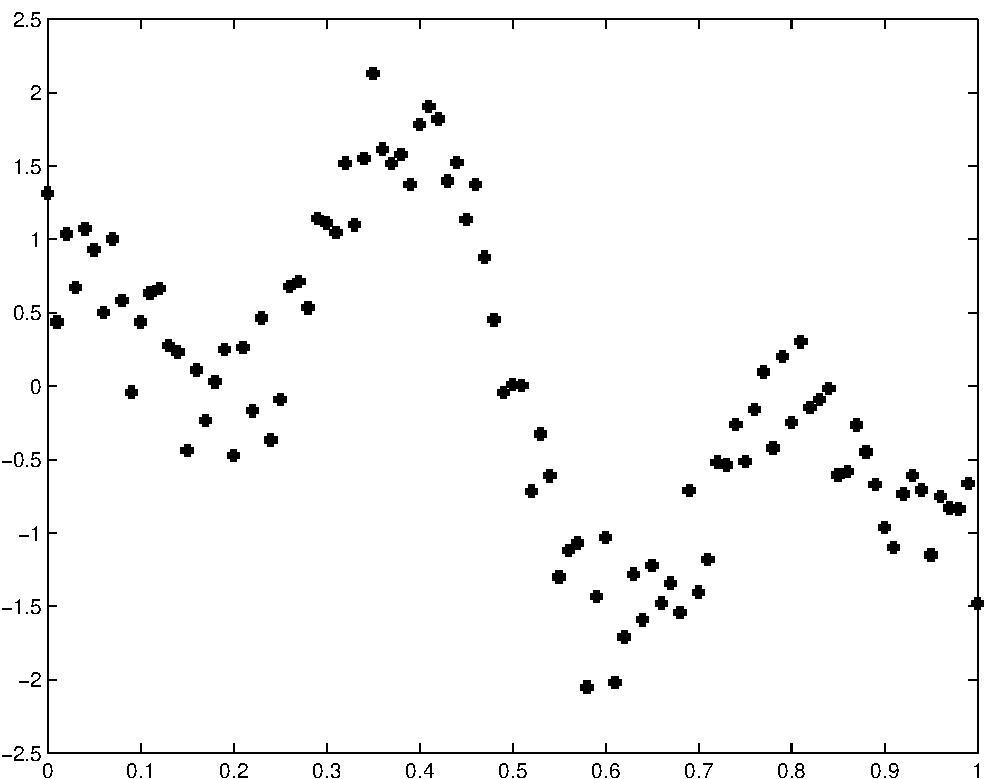
\includegraphics[width=55mm,height=35mm]
{demRegressData}
\end{center}

  \item<2-> Gaussian process prior (RBF kernel) 
%\begin{figure}[ht]
\begin{center}
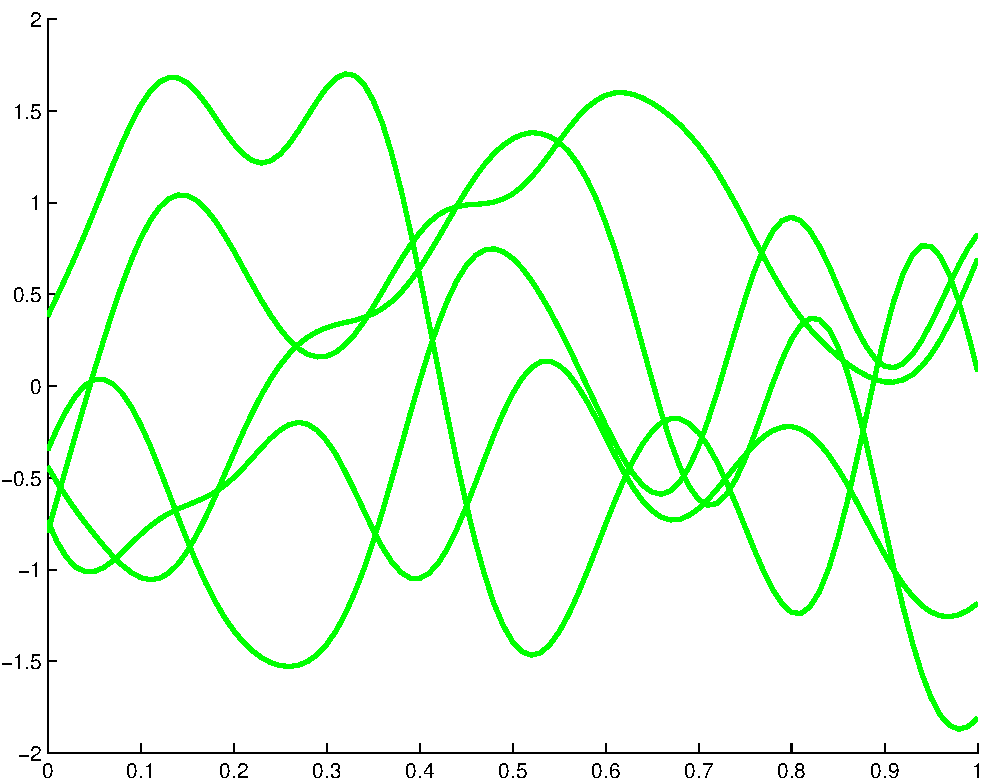
\includegraphics[width=55mm,height=35mm]
{demRegressSamPrior}
\end{center}
%\end{figure}

  \end{itemize}
}

\frame
{
  \frametitle{Gaussian Processes for Bayesian Regression}
  \begin{itemize}
  \item Posterior 

\begin{center}
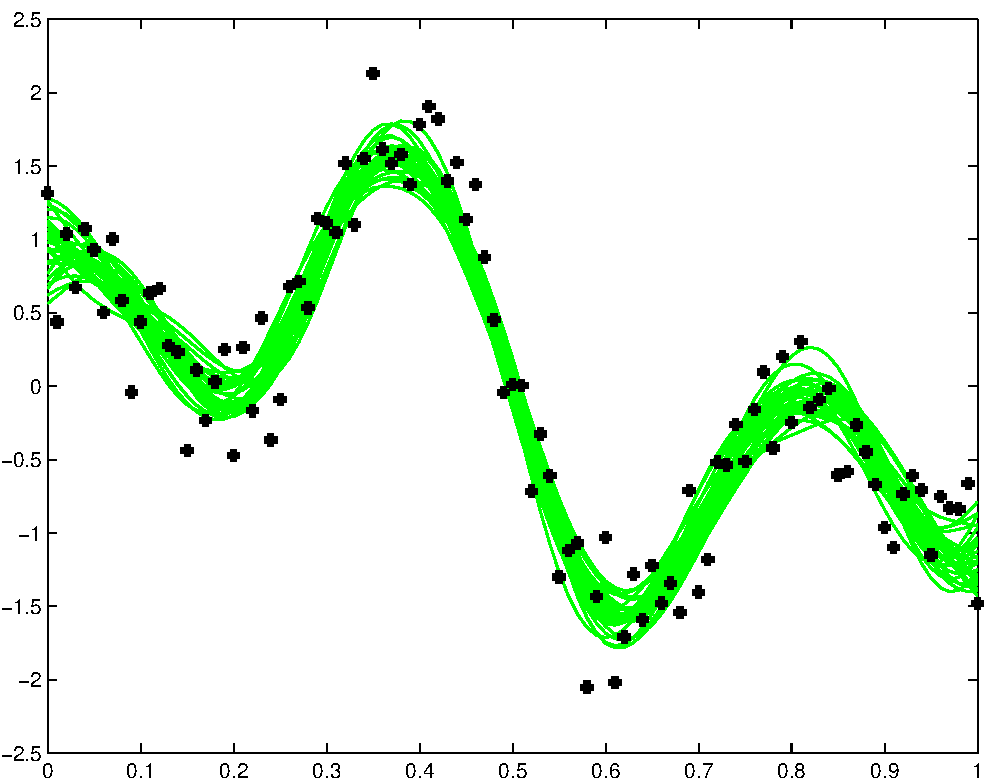
\includegraphics[width=55mm,height=40mm]
{demRegressTreuGPSamples}
\end{center}

  \end{itemize}
}

\frame
{
  \frametitle{Gaussian Processes for non-Gaussian Likelihoods}

  \begin{itemize}
  \item If the likelihood $p(\bfy|\bff)$ is non-Gaussian 
        (nonlinear model w.r.t. $\bff$ or non Gaussian noise)  
         computations become \textcolor{red}{intractable}

  \item Examples of such likelihoods arise in:   
 
 \begin{itemize}
  \item  Classification problems

   \item Non-linear differential equations 

 \end{itemize}


  \item Approximations need to be considered 

     
  \item  MCMC offers a general framework for inference 
             \begin{itemize}
             \item It is applied independently from the form of
                       the likelihood  
             \item Gives exact inference in the limit of many samples  

             \item Can be used to validate deterministic
             approximations  
            
             \end{itemize}

  \end{itemize}
}


\frame
{
  \frametitle{MCMC for Gaussian Processes}

The \textcolor{red}{Metropolis-Hastings} algorithm 

  \begin{itemize}

  \item Initialize $\bff^{(0)}$

  \item  Form a Markov chain. Use a proposal distribution 
            $Q(\bff^{(t+1)}|\bff^{(t)})$ and accept with the M-H step 

$$
\min \left(1,\frac{p(\bfy|\bff^{(t+1)}) p(\bff^{(t+1)})}
{p(\bfy|\bff^{(t)}) p(\bff^{(t)})}  \frac{Q(\bff^{(t)}|\bff^{(t+1)})}
{Q(\bff^{(t+1)}|\bff^{(t)})} \right)
$$ 

\item $\bff$ can be very \textcolor{red}{high dimensional} (hundreds of points) 

\item How do we choose the proposal $Q(\bff^{(t+1)}|\bff^{(t)})$? 

\begin{itemize}
\item  Can we use the \textcolor{red}{GP prior $p(\bff)$} as the proposal?
\end{itemize}

%\item What about using the \textcolor{red}{GP prior $p(\bff)$} as the proposal 
%  \begin{itemize}
% 
%    \item we will get 0 acceptance rate 
%   \item \textcolor{red}{BUT:} the prior samples functions with the
%       appropriate smoothing constraints
 
\end{itemize}

}


\frame
{
  \frametitle{Sampling using control points}

\begin{itemize}
\item Separate the points in $\bff$ into two groups: 

\begin{itemize}

   \item few \textcolor{red}{control} points $\bff_c$  
   \item and the large majority of the \textcolor{red}{remaining} 
      points $\bff_{\rho} = \bff \setminus \bff_c$  

\end{itemize}

\item Sample the control points $\bff_c$ using a proposal 
$q(\bff_c^{(t+1)}|\bff_c^{(t)})$ 

\item Sample the remaining points $\bff_{\rho}$ using the
conditional GP prior $p(\bff_{\rho}^{(t+1)}|\bff_c^{(t+1)})$ 

\item The whole proposal is
$$
Q(\bff^{(t+1)}|\bff^{(t)}) =  p(\bff_{\rho}^{(t+1)} | \bff_{c}^{(t+1)})
q(\bff_{c}^{(t+1)} | \bff_c^{(t)})
$$

\item  Its like sampling from the \textcolor{red}{prior} $p(\bff)$  
      but \textcolor{red}{imposing random walk}
      behaviour  through the control points 
\end{itemize}
}


\frame
{
  \frametitle{Sampling using control points: Regression-Examples}

Sample 121 points using 10 control points

\begin{center}
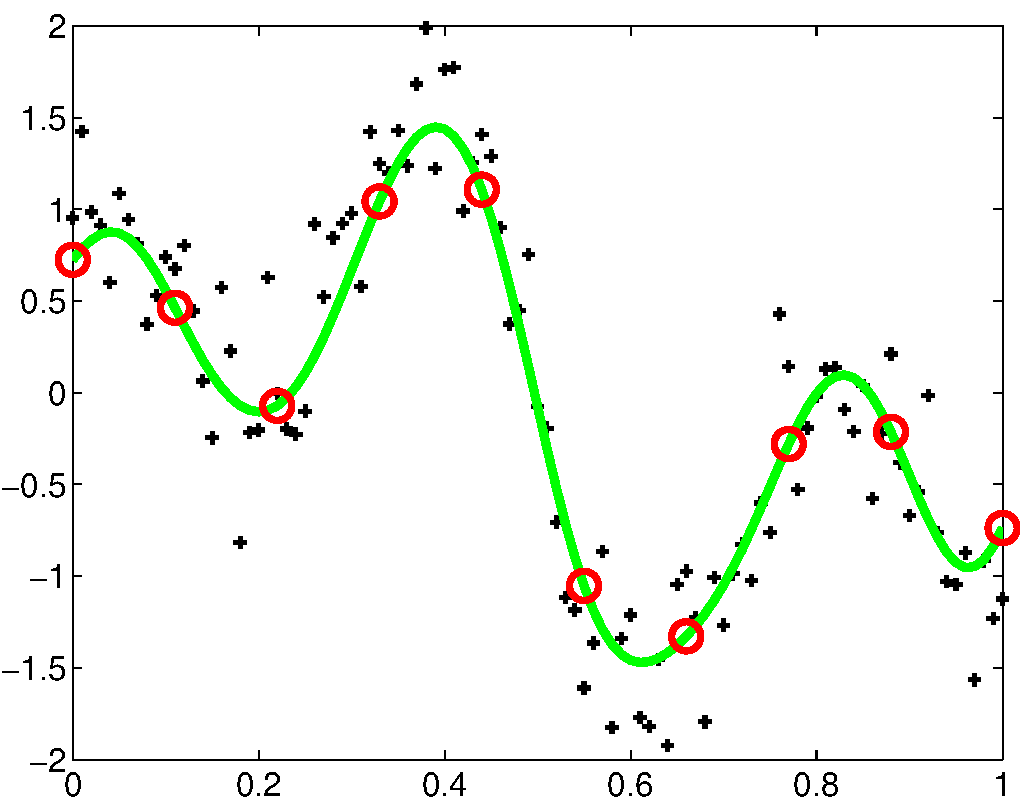
\includegraphics[width=75mm,height=60mm]
{demRegressCurrent11000.pdf}
\end{center}

}


\frame
{
  \frametitle{Sampling using control points: Regression-Examples}

Sample 121 points using 10 control points

\begin{center}
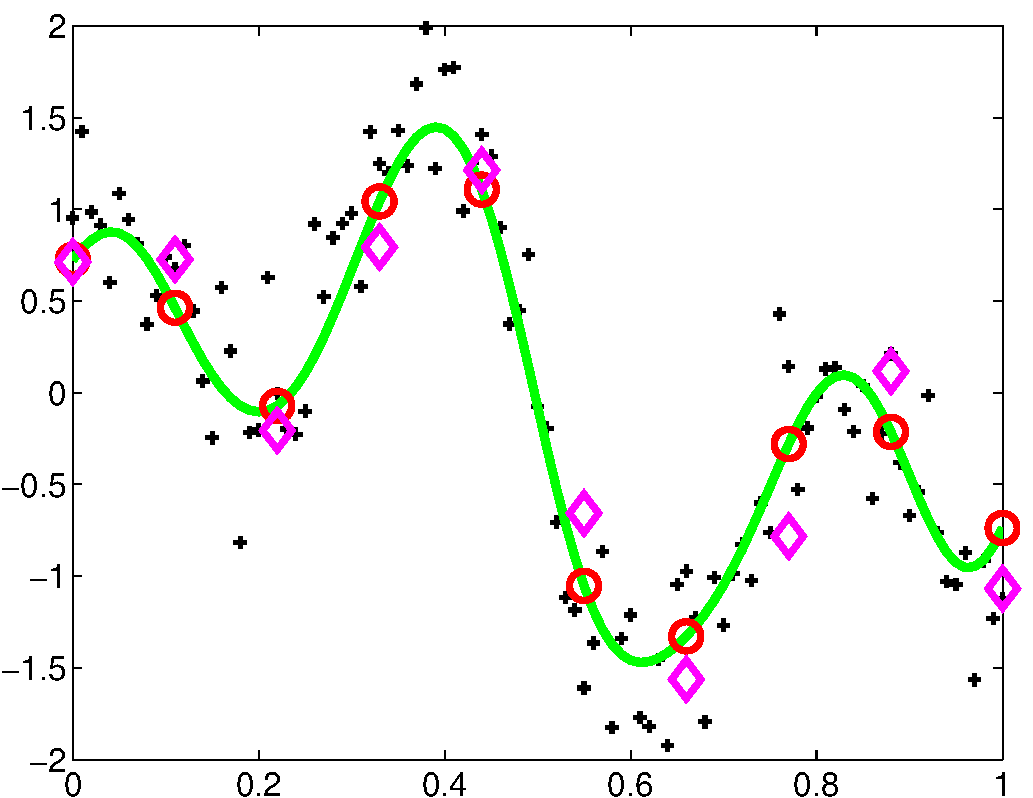
\includegraphics[width=75mm,height=60mm]
{demRegressNewControls11000.pdf}
\end{center}

}

\frame
{
  \frametitle{Sampling using control points: Regression-Examples}

Sample 121 points using 10 control points

\begin{center}
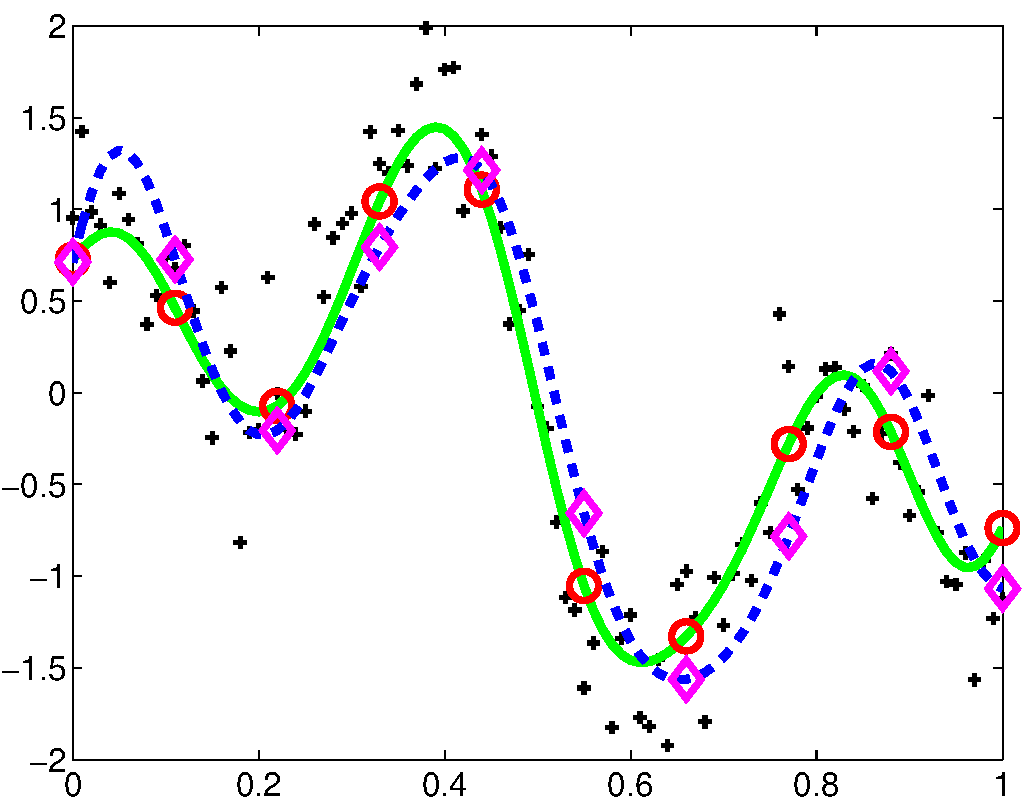
\includegraphics[width=75mm,height=60mm]
{demRegressFinal11000.pdf}
\end{center}


}


\frame
{
  \frametitle{Sampling using control points: Regression-Examples}


Sample 121 points using 10 control points

\begin{center}
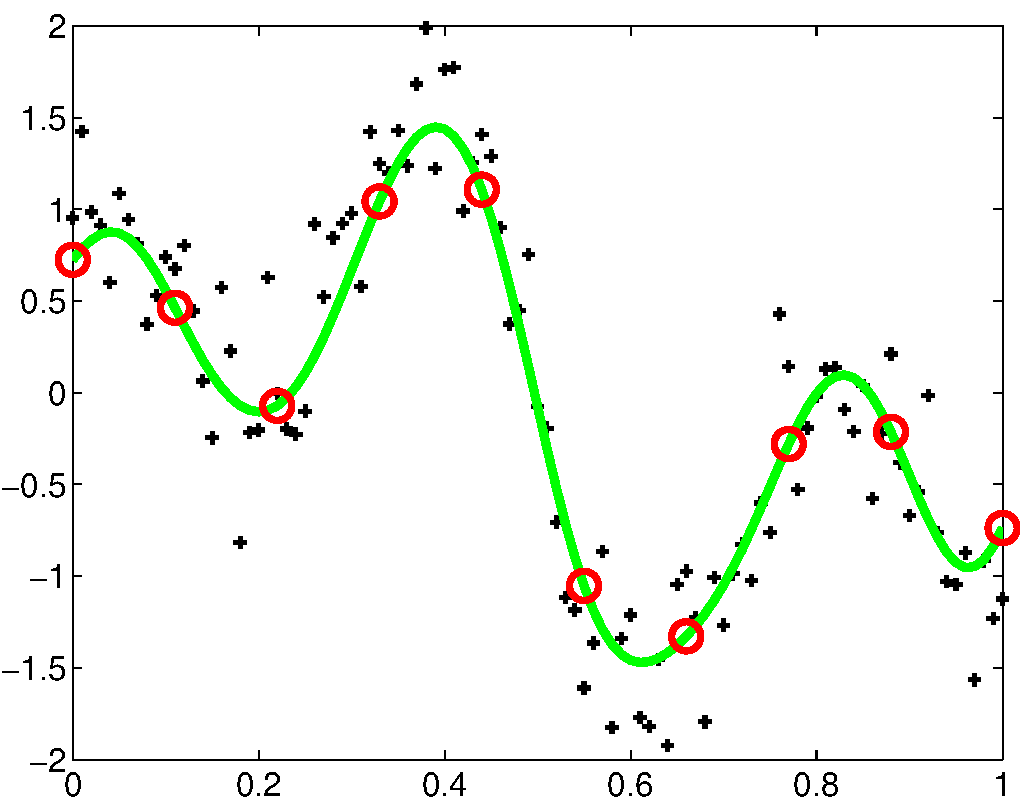
\includegraphics[width=75mm,height=60mm]
{demRegressCurrent10000.pdf}
\end{center}

}


\frame
{
  \frametitle{Sampling using control points: Regression-Examples}


Sample 121 points using 10 control points

\begin{center}
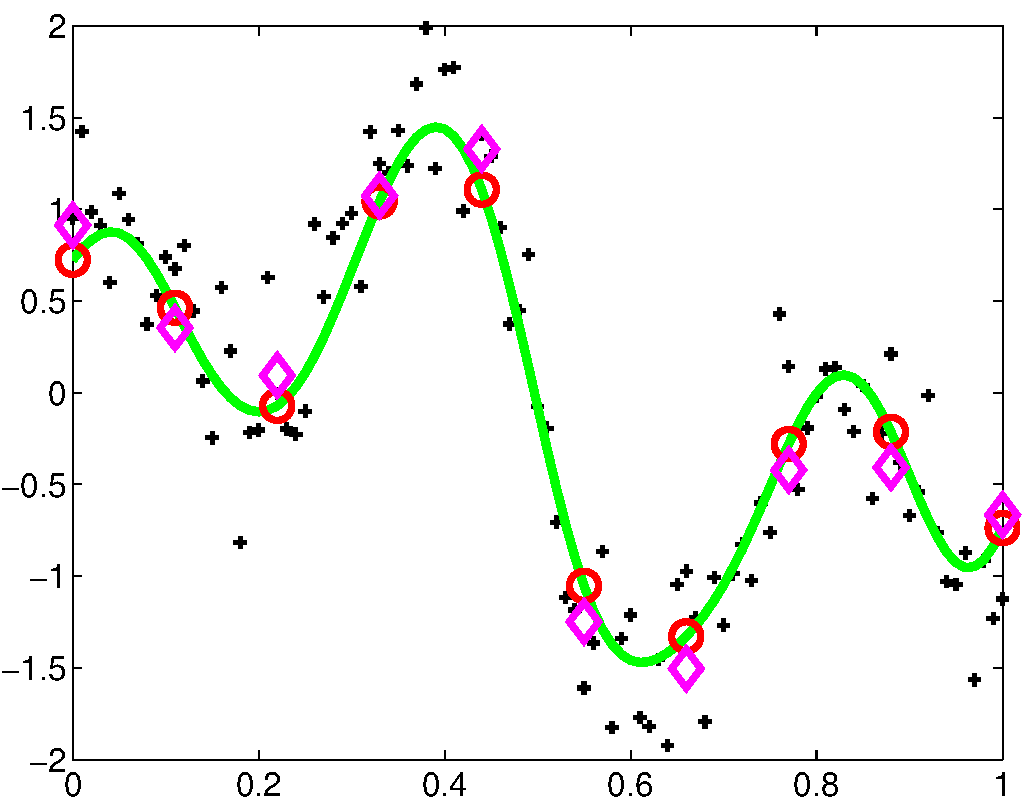
\includegraphics[width=75mm,height=60mm]
{demRegressNewControls10000.pdf}
\end{center}

}

\frame
{
  \frametitle{Sampling using control points: Regression-Examples}


Sample 121 points using 10 control points


\begin{center}
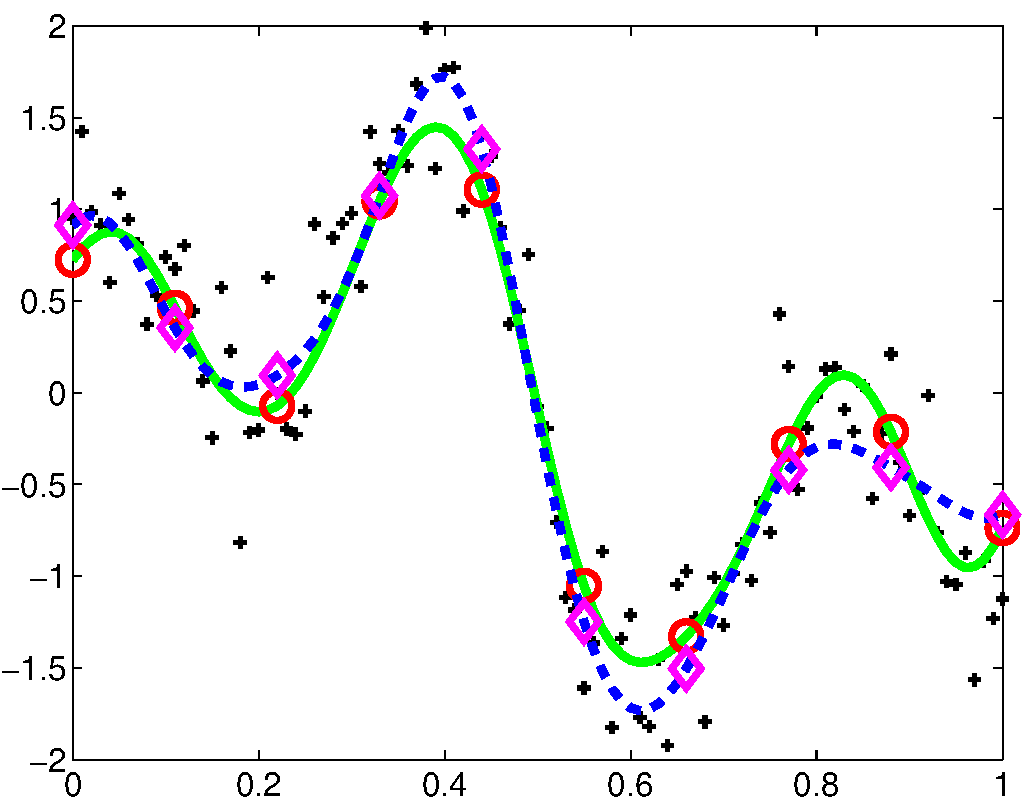
\includegraphics[width=75mm,height=60mm]
{demRegressFinal10000.pdf}
\end{center}

}

\frame
{
 \frametitle{Sampling using control points}

Few samples drawn during MCMC 

\begin{center}
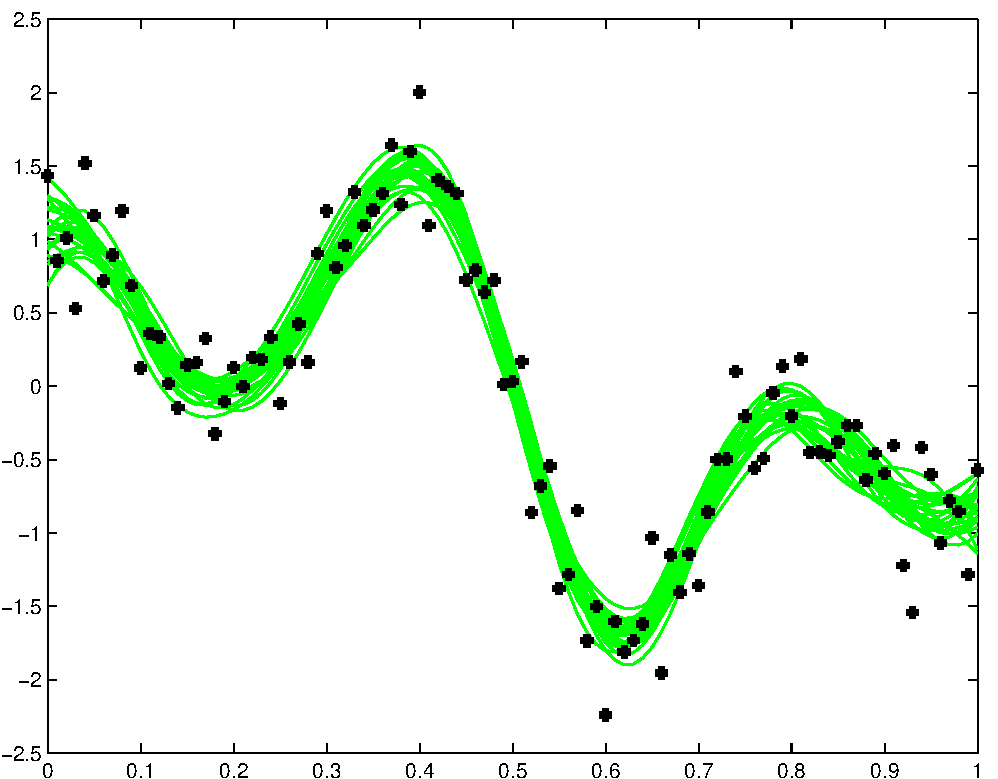
\includegraphics[width=55mm,height=40mm]
{demRegressMCMCSamples}
\end{center}

}

\frame
{
 \frametitle{Sampling using control points: Adaption of the proposal}

Issues that need to be resolved during the burn in MCMC phase

\begin{itemize}
\item \textcolor{red}{Number} of control points
\item \textcolor{red}{Which points} should be used as control points
\item Improve the \textcolor{red}{acceptance rate} by 
\begin{itemize}

\item Adapting the variance of  $q(\bff_{c}^{(t+1)} | \bff_c^{(t)})$  
      during the burn in period 

\item Sampling the control points in a block-wise manner (keep some of them
  fixed when you sample others)

\end{itemize}
\end{itemize}

For the transcription factor modelling application there are natural 
choices for all the above issues. In the data we have considered so
far we only need to adapt the variances of  $q(\bff_{c}^{(t+1)} | \bff_c^{(t)})$

}


\frame
{

\frametitle{Transcriptional regulation}

\begin{itemize}

\item \textcolor{red}{Data:} Gene expression levels $\bfy = (y_{jt})$ of $N$
      genes at $T$ times
      %. Assuming Gaussian noise the \textcolor{red}{likelihood} is   

\item \textcolor{red}{Goal:} We suspect/know that a certain protein
            regulates ( i.e.\ is a transcription factor (TF) ) these genes and we wish to model this
            relationship  
 
\item \textcolor{red}{Model:} Use a differential equation (Barenco et al. [2006];
  Rogers et. al. [2007])     

$$
\frac{d y_j (t)} {d t} =
B_j + S_j g(f(t)) - D_j y_j(t)
$$

\item where 

$t$ - time

$y_j(t)$ - expression of the $j$th gene %at time $t$

$f(t)$ - concentration of the transcription factor protein 

$D_j$ - decay rate 

$B_j$ - basal rate

$S_j$ - Sensitivity 

%$g$ - the activation function of the protein $f(t)$ 
%  (e.g.\ linear or the Michaelis-Menten kinetic equation)

\end{itemize}


}



%\frame
%{
% \frametitle{Transcriptional regulation using Gaussian processes}
%
%
%\begin{itemize}
%\item Model of transcriptional regulation (Barenco et al. [2006];
%  Rogers et. al. [2007])
%
%$$
%\frac{d y_j (t)} {d t} =
%B_j + S_j g(f(t)) - D_j y_j(t)
%$$
%
%\item where 
%
%$y_j(t)$ - expression of the $j$th gene at time $t$
%
%$f(t)$ - concentration of the transcription factor protein 
%
%$D_j$ - decay rate 
%
%$B_j$ - basal rate 
%
%$S_j$ - Sensitivity 
%
%$g$ - the activation function of the protein $f(t)$ 
%  (e.g.\ linear or the Michaelis-Menten kinetic equation)
%
%
%\item Solve the equation
%$$
%y_j(t) = \frac{B_j}{D_j} +  A_j \exp(D_j t) +
%S_j \exp(-D_j t) \int_{0}^t g(f(u)) \exp(D_j u) du
%$$
%
%\end{itemize}
%
%}



\frame
{
 \frametitle{Transcriptional regulation using Gaussian processes}


\begin{itemize}
\item Solve the equation % Generally the solution is not analytically obtained 
$$
y_j(t) = \frac{B_j}{D_j} +  A_j \exp(-D_j t) +
S_j \exp(-D_j t) \int_{0}^t g(f(u)) \exp(D_j u) du
$$

\item Apply numerical integration using a very dense grid $(u_i)_{i=1}^P$ and  $\bff = (f_i(u_i))_{i=1}^P$ 
%and apply numerical integration
$$
y_j(t) \simeq \frac{B_j}{D_j} +  A_j \exp(-D_j t) +
S_j \exp(-D_j t) \sum_{p=1}^{P_t} w_p g(f_p) \exp(D_j u_p)
$$
Assuming Gaussian noise for the observed gene expressions $\{y_{jt}\}$, the ODE
defines the likelihood $p(\bfy|\bff)$
%where the weights $w_p$ are given e.g.\ by the composite Simpson rule (the
%simple Simpson (P=3) integrates exactly polynomials up to cubic
%degree)
\item \textcolor{red}{Bayesian inference:} Assume a GP prior for the
 transcription factor $\bff$ and apply MCMC to infer 
 $(\bff, \{A_j,B_j,D_j,S_j\}_{j=1}^N)$

\begin{itemize}
%
%\item Gaussian process prior for $\bff$
%
%\item Gamma vague prior for $(A_j,B_j,D_j,S_j)$
%
%\item Use MCMC to sample  $(\bff, \{A_j,B_j,D_j,S_j\}_{j=1}^N)$

\item $\bff$ is inferred in a \textcolor{red}{continuous} manner ($P \gg T$)

\end{itemize}

%\begin{itemize}
%
%\item Gaussian process prior for $\bff$
%
%\item Gamma vague prior for $(A_j,B_j,D_j,S_j)$
%
%\item Use MCMC to sample  $(\bff, \{A_j,B_j,D_j,S_j\}_{j=1}^N)$
%
%\item $\bff$ is inferred in a \textcolor{red}{continuous} manner ($P \gg T$)
%
%\end{itemize}


\end{itemize}

}




%\frame
%{
% \frametitle{Transcriptional regulation: Fit the model to data}
%
%$$
%\mu_j(t) = \frac{B_j}{D_j} +  A_j \exp(D_j t) +
%S_j \exp(-D_j t) \sum_{p=1}^{P_t} w_p g(f_p) \exp(D_j u_p)
%$$
%\begin{itemize}
%
%\item \textcolor{red}{Data:} gene expression levels $\bfy = (y_{jt})$ of $N$
%      genes at $T$ times. Assuming Gaussian noise the 
%      \textcolor{red}{likelihood} is   
%
%$$
%p(\bfy |\bff, \{A_j,D_j,B_j,S_j\} ) 
%=\prod_{j=1}^N \prod_{t=1}^T N(y_{jt} | \mu_{jt}, \sigma_{jt}^2) 
%$$  
%    
%
%\item \textcolor{red}{Bayesian inference:} Estimate the transcription factor $\bff$ and the gene
%parameters $(A_j,B_j,D_j,S_j)$
%
%\begin{itemize}
%
%\item Gaussian process prior for $\bff$
%
%\item Gamma vague prior for $(A_j,B_j,D_j,S_j)$
% 
%\item Use MCMC to sample  $(\bff, \{A_j,B_j,D_j,S_j\}_{j=1}^N)$
%
%\item $\bff$ is inferred in a \textcolor{red}{continuous} manner ($P \gg T$)
%
%\end{itemize}
%
%\end{itemize}
%
%}





\frame
{
 

\frametitle{Results in E.coli data: Rogers, Khanin and Girolami (2007)}

\begin{itemize}
\item  One transcription factor (lexA) that acts as a repressor. We
  consider the Michaelis-Menten kinetic equation  
$$
\frac{d y_j (t)} {d t} =
B_j + S_j \frac{1}{\exp(f(t)) + \gamma_j} - D_j y_j(t)
$$

\item We have 14 genes (5 kinetic parameters each)

\item Gene expressions are available for $T=6$ time slots 

\item TF ($\bff$) is discretized using 121 points

\item MCMC details: 
\begin{itemize}
\item 6 control points are used (placed in a equally spaced grid)    
\item Running time was  5 hours for 2 million sampling iterations plus
      burn in 
\item Acceptance rate for $\bff$ after burn in was between 
      $15\%-25\%$ 
\end{itemize}

\end{itemize}

}


\frame
{
 
\frametitle{Results in E.coli data:  Predicted gene expressions}

\begin{figure}
\begin{center}
\begin{tabular}{ccc}
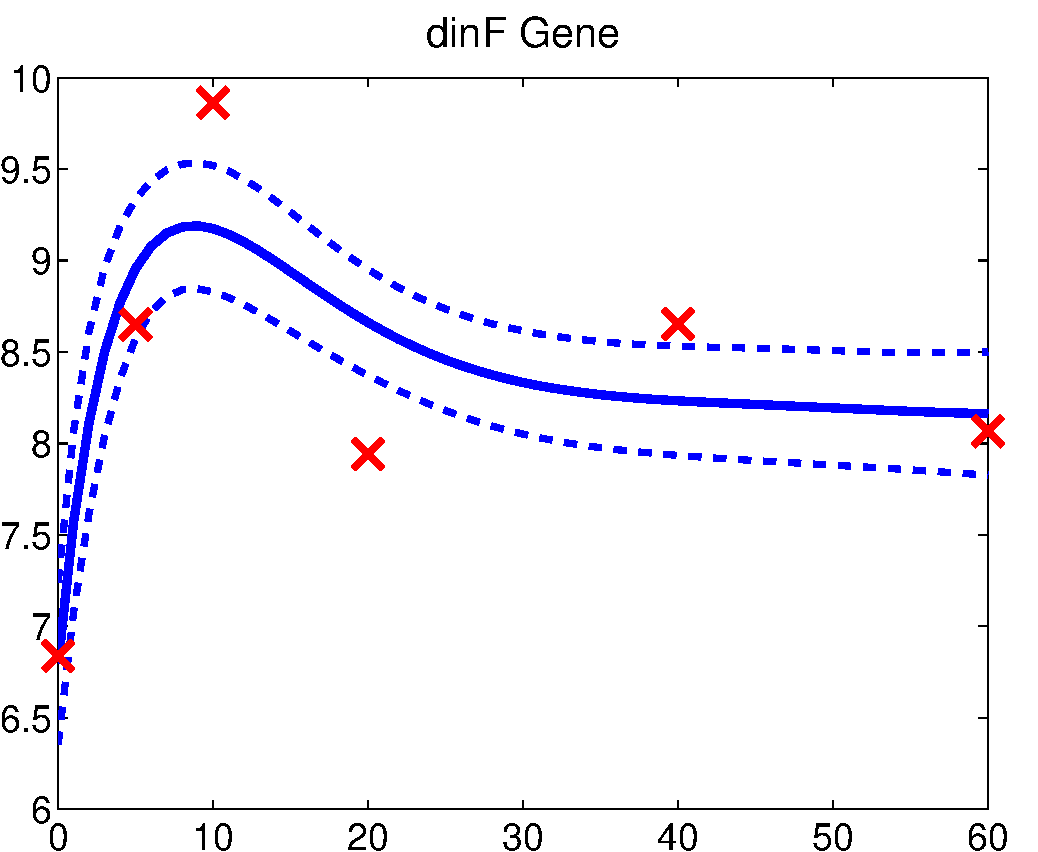
\includegraphics[width=35mm,height=33mm]
{demEcoliNoMCMC4RbfexpMichMentenRepres_ExprsProfile_Rep1_Gene1.pdf}&
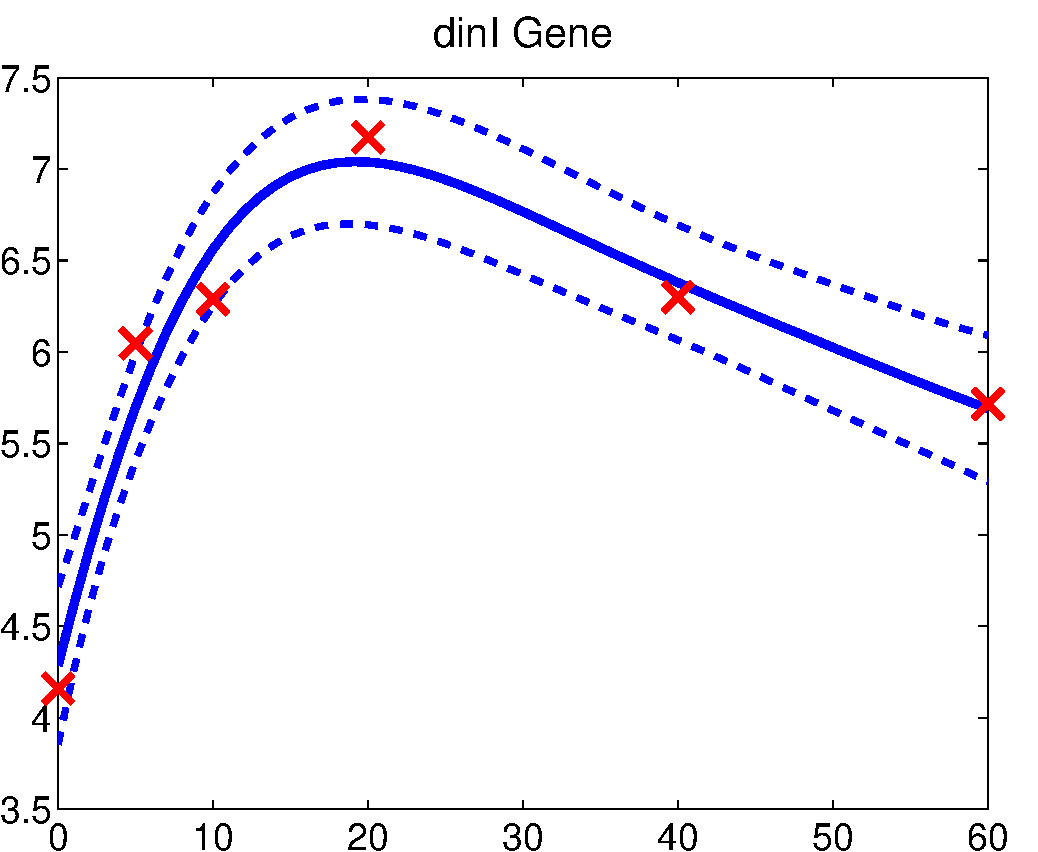
\includegraphics[width=35mm,height=33mm]
{demEcoliNoMCMC4RbfexpMichMentenRepres_ExprsProfile_Rep1_Gene2.pdf}&
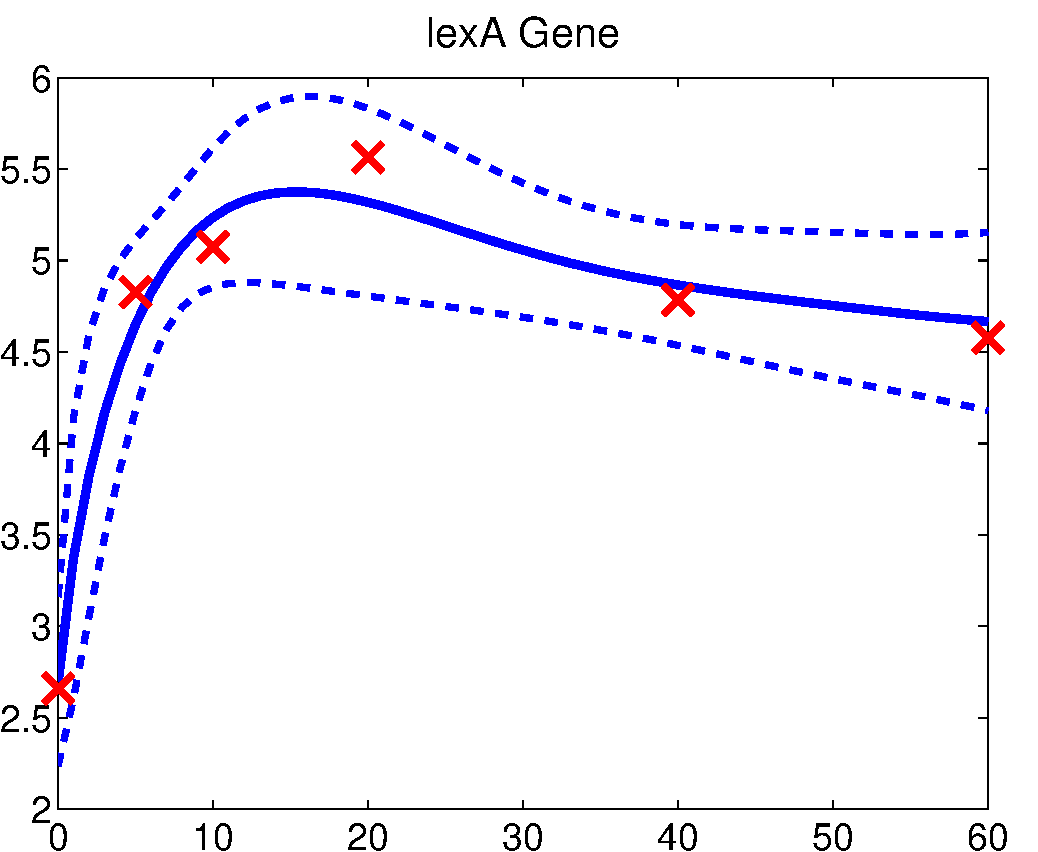
\includegraphics[width=35mm,height=33mm]
{demEcoliNoMCMC4RbfexpMichMentenRepres_ExprsProfile_Rep1_Gene3.pdf} \\
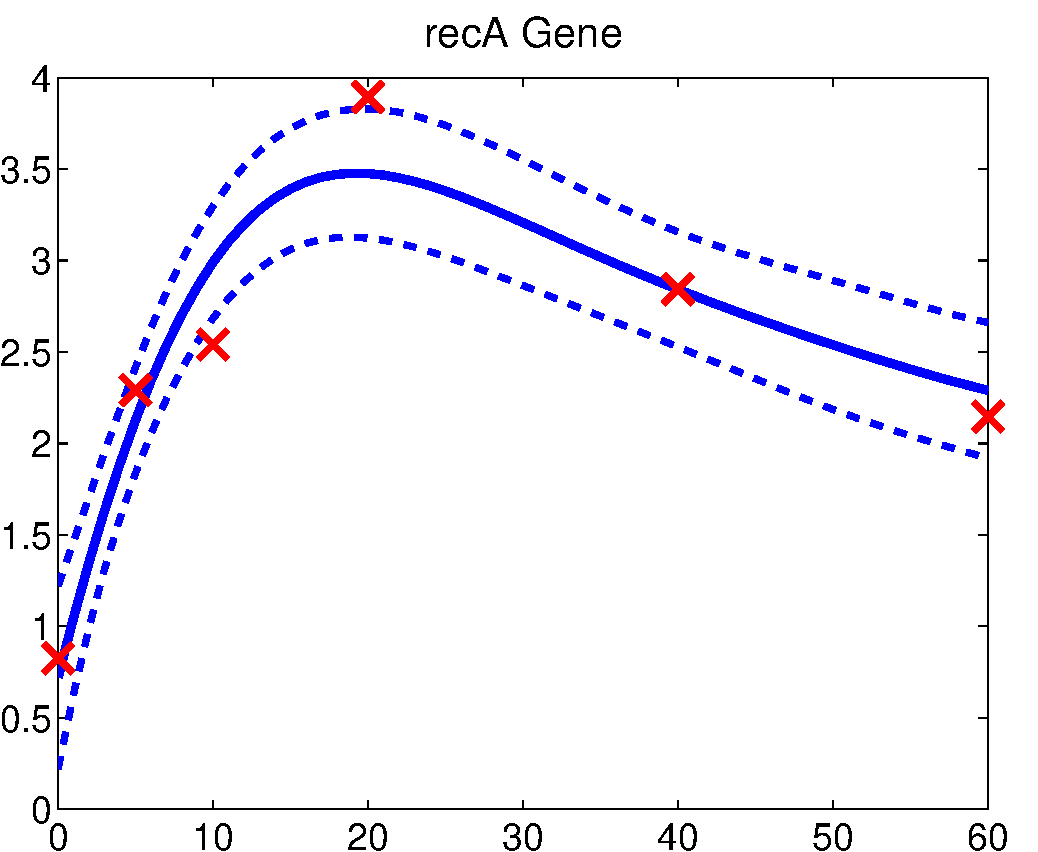
\includegraphics[width=35mm,height=33mm]
{demEcoliNoMCMC4RbfexpMichMentenRepres_ExprsProfile_Rep1_Gene4.pdf}&
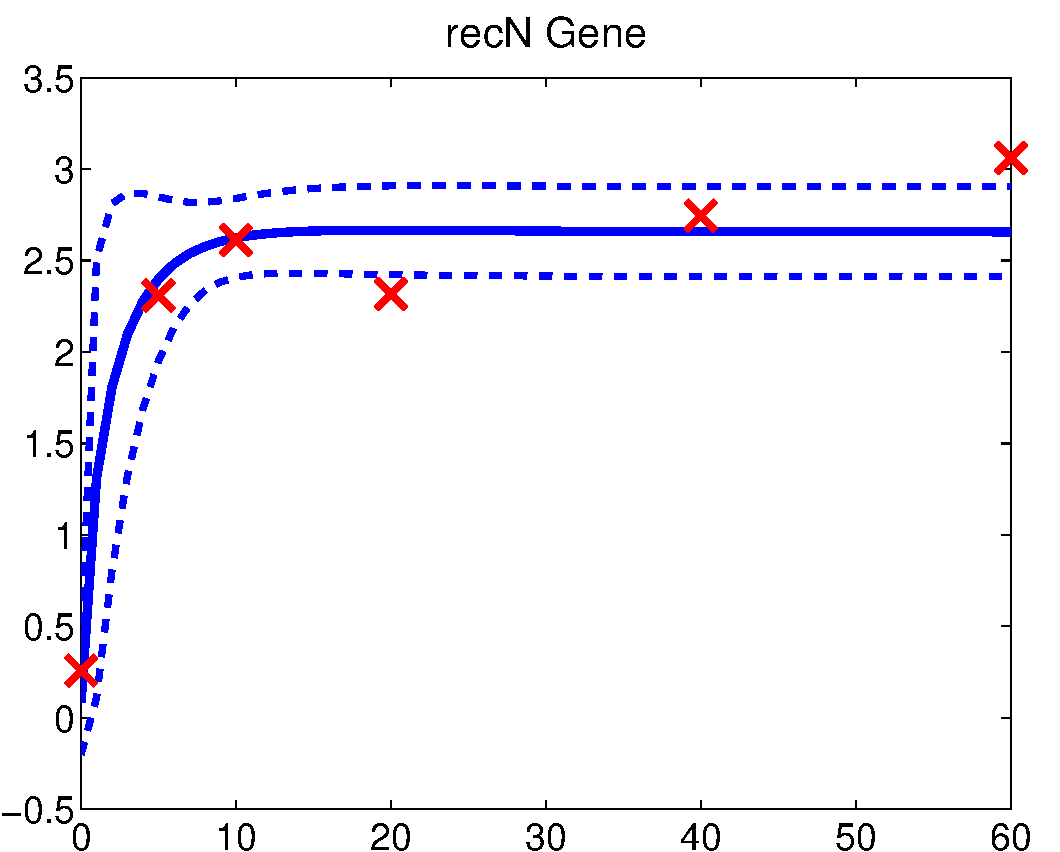
\includegraphics[width=35mm,height=33mm]
{demEcoliNoMCMC4RbfexpMichMentenRepres_ExprsProfile_Rep1_Gene5.pdf}&
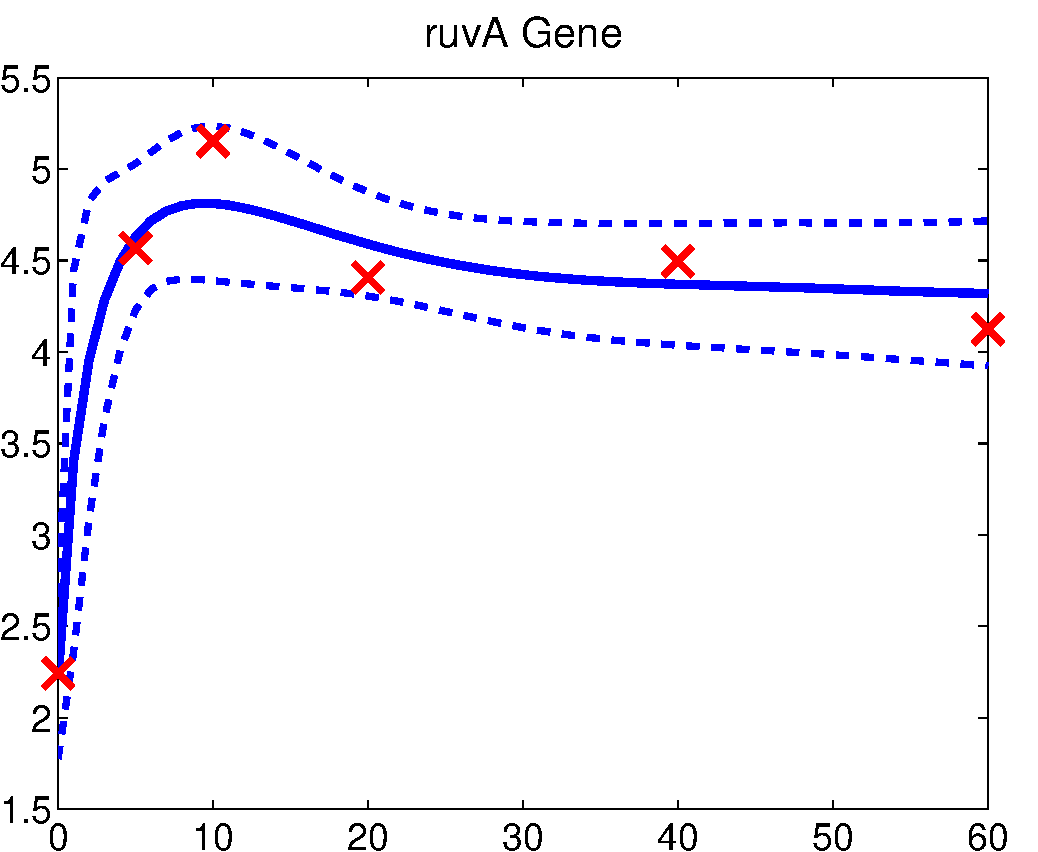
\includegraphics[width=35mm,height=33mm]
{demEcoliNoMCMC4RbfexpMichMentenRepres_ExprsProfile_Rep1_Gene6.pdf}
\end{tabular}
\end{center}
\end{figure}


}



\frame
{
 
\frametitle{Results in E.coli data: Predicted gene expressions}


\begin{figure}
\begin{center}
\begin{tabular}{ccc}
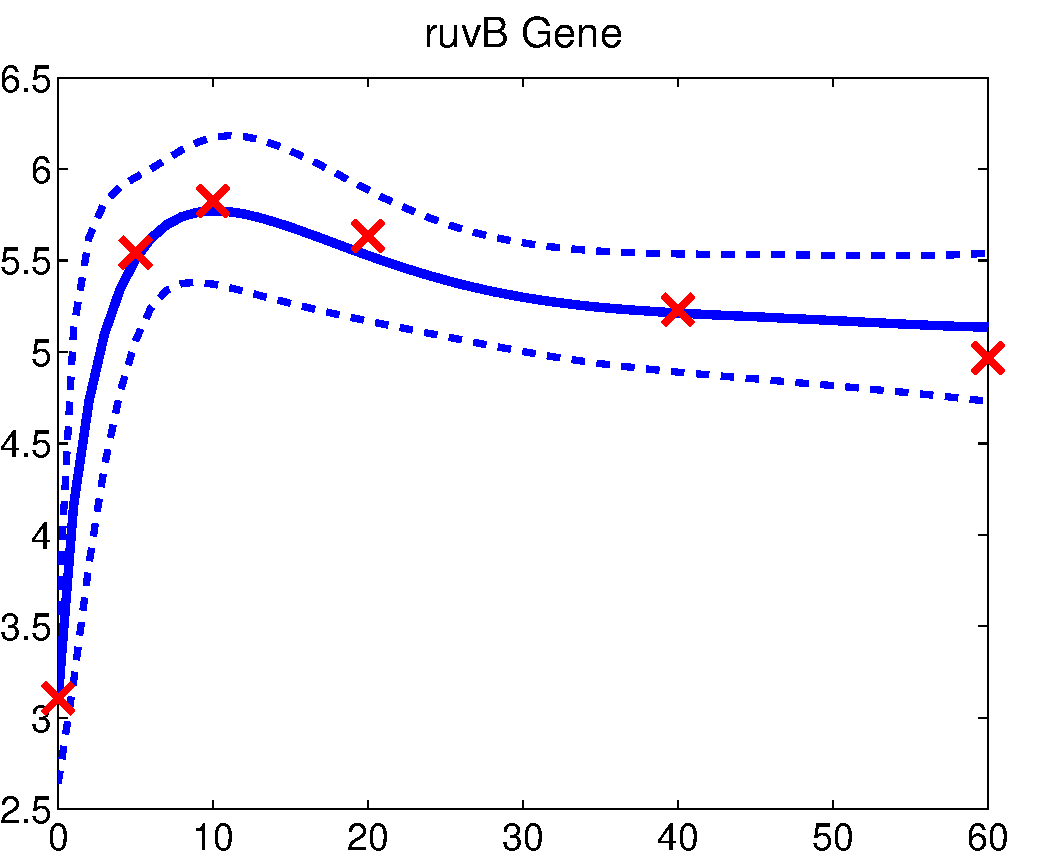
\includegraphics[width=35mm,height=33mm]
{demEcoliNoMCMC4RbfexpMichMentenRepres_ExprsProfile_Rep1_Gene7.pdf}&
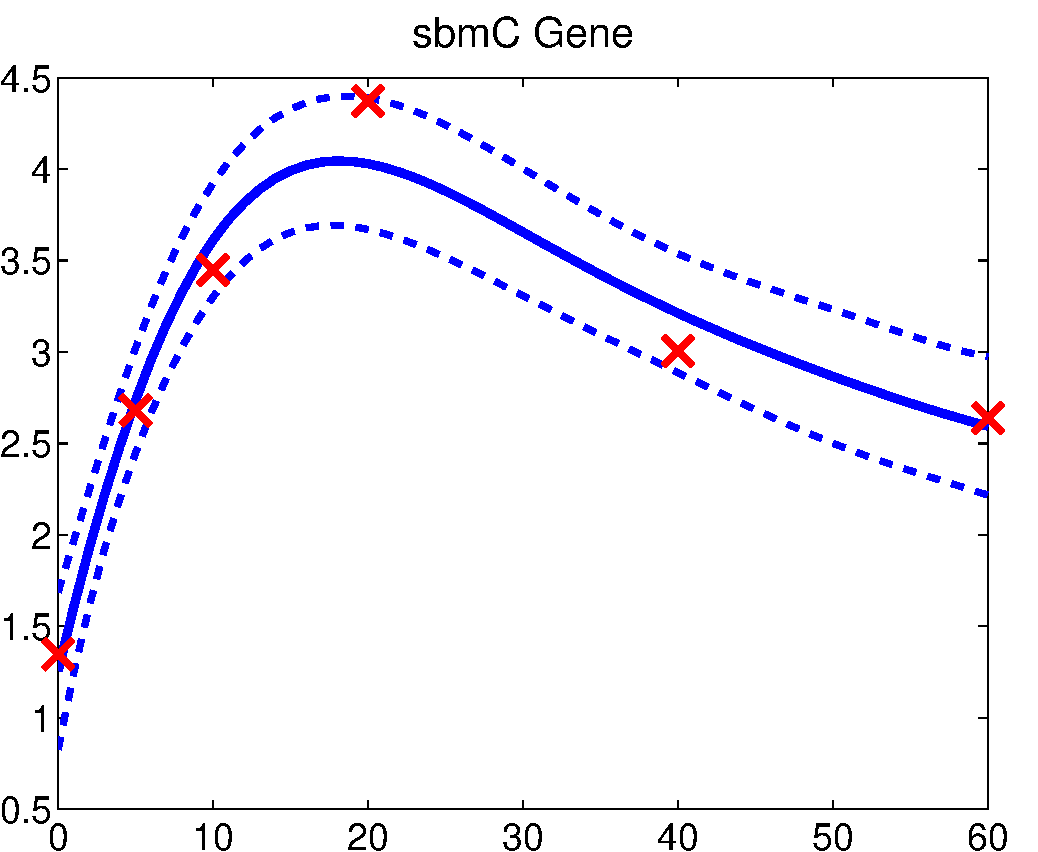
\includegraphics[width=35mm,height=33mm]
{demEcoliNoMCMC4RbfexpMichMentenRepres_ExprsProfile_Rep1_Gene8.pdf}&
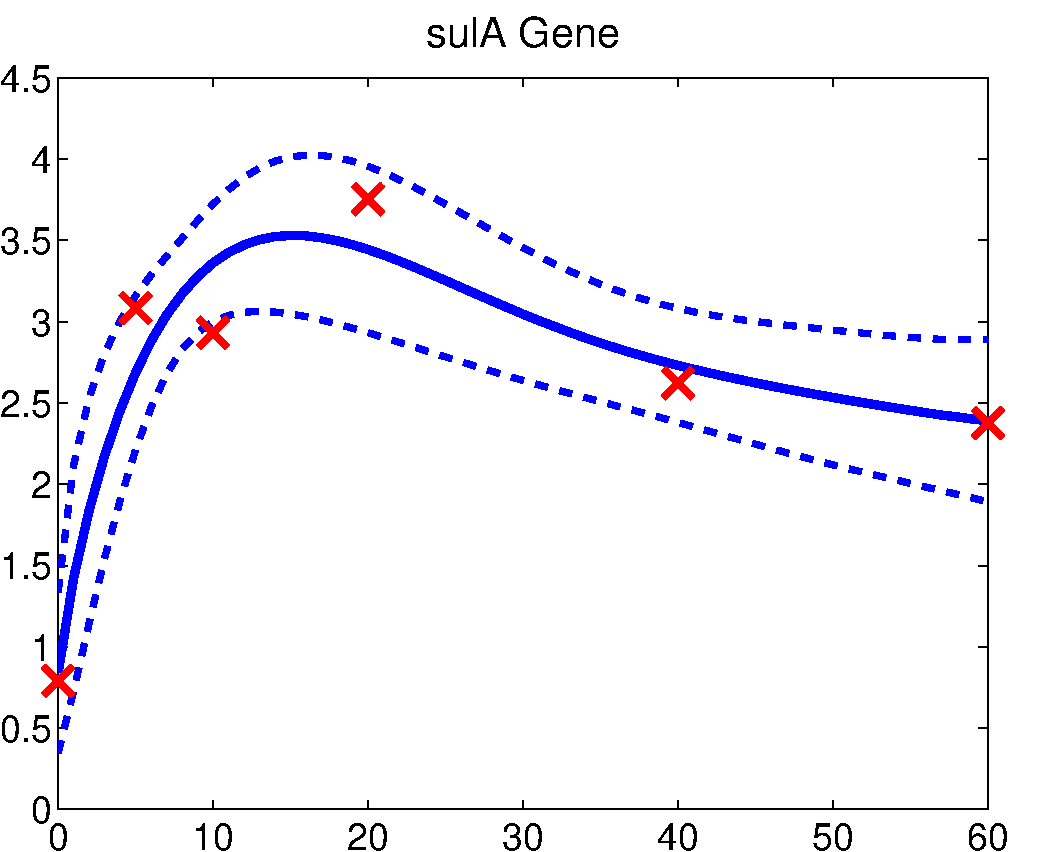
\includegraphics[width=35mm,height=33mm]
{demEcoliNoMCMC4RbfexpMichMentenRepres_ExprsProfile_Rep1_Gene9.pdf} \\
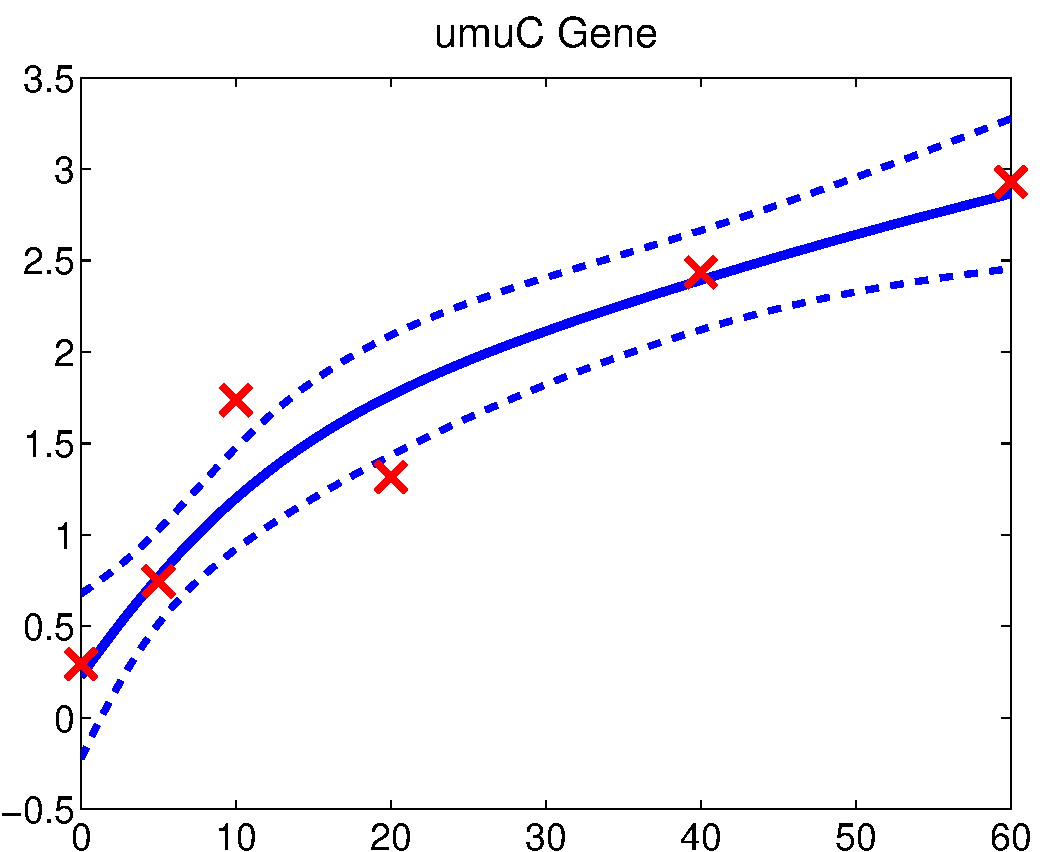
\includegraphics[width=35mm,height=33mm]
{demEcoliNoMCMC4RbfexpMichMentenRepres_ExprsProfile_Rep1_Gene10.pdf}&
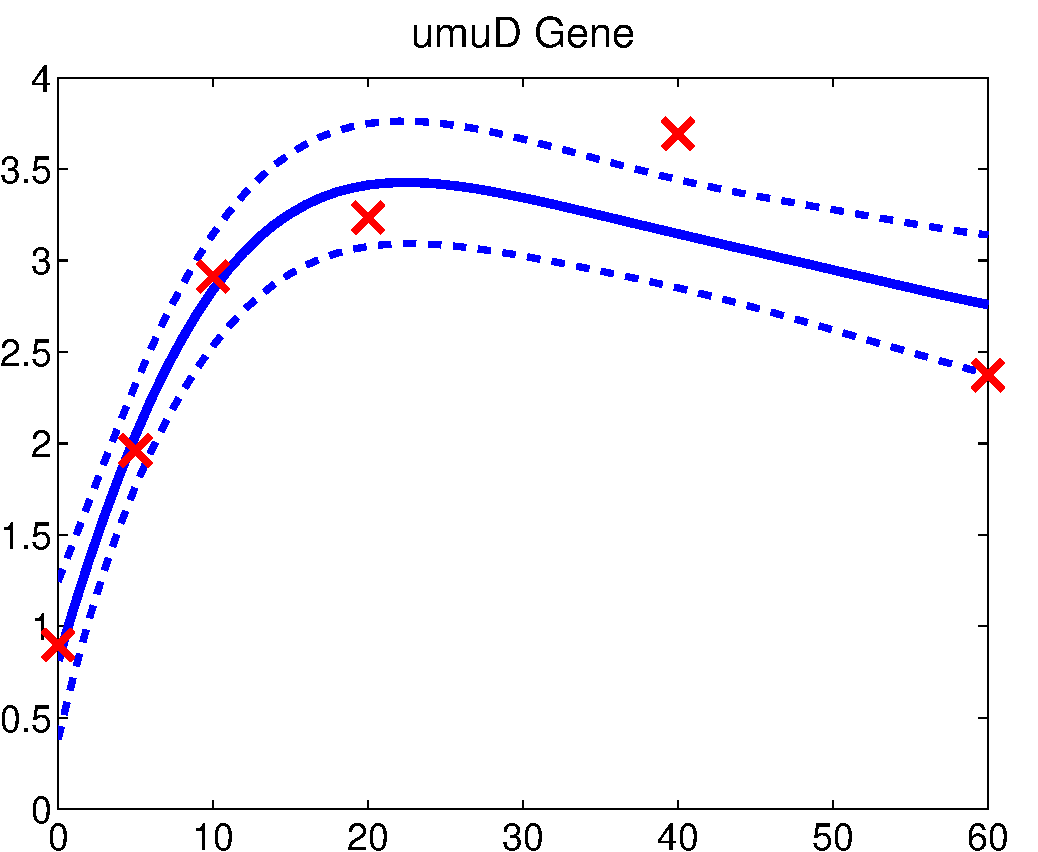
\includegraphics[width=35mm,height=33mm]
{demEcoliNoMCMC4RbfexpMichMentenRepres_ExprsProfile_Rep1_Gene11.pdf}&
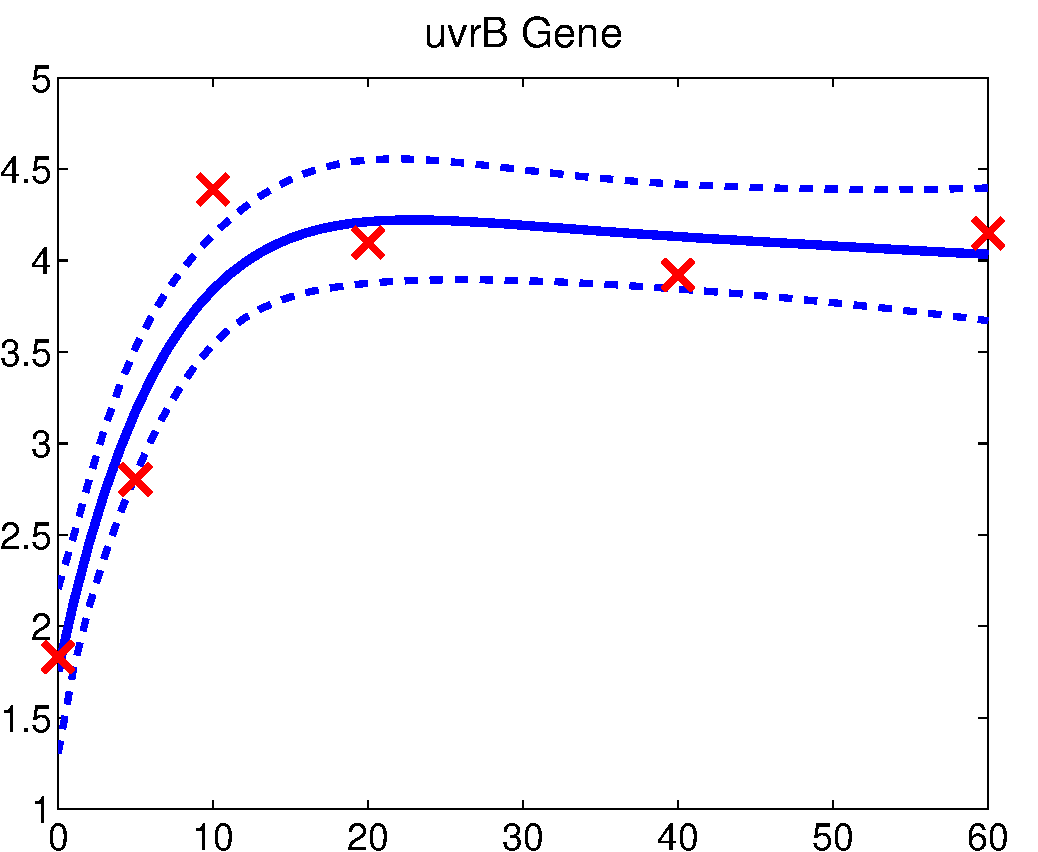
\includegraphics[width=35mm,height=33mm]
{demEcoliNoMCMC4RbfexpMichMentenRepres_ExprsProfile_Rep1_Gene12.pdf}
\end{tabular}
\end{center}
\end{figure}


}


\frame
{
 
\frametitle{Results in E.coli data: Predicted gene expressions}


\begin{figure}
\begin{center}
\begin{tabular}{cc}
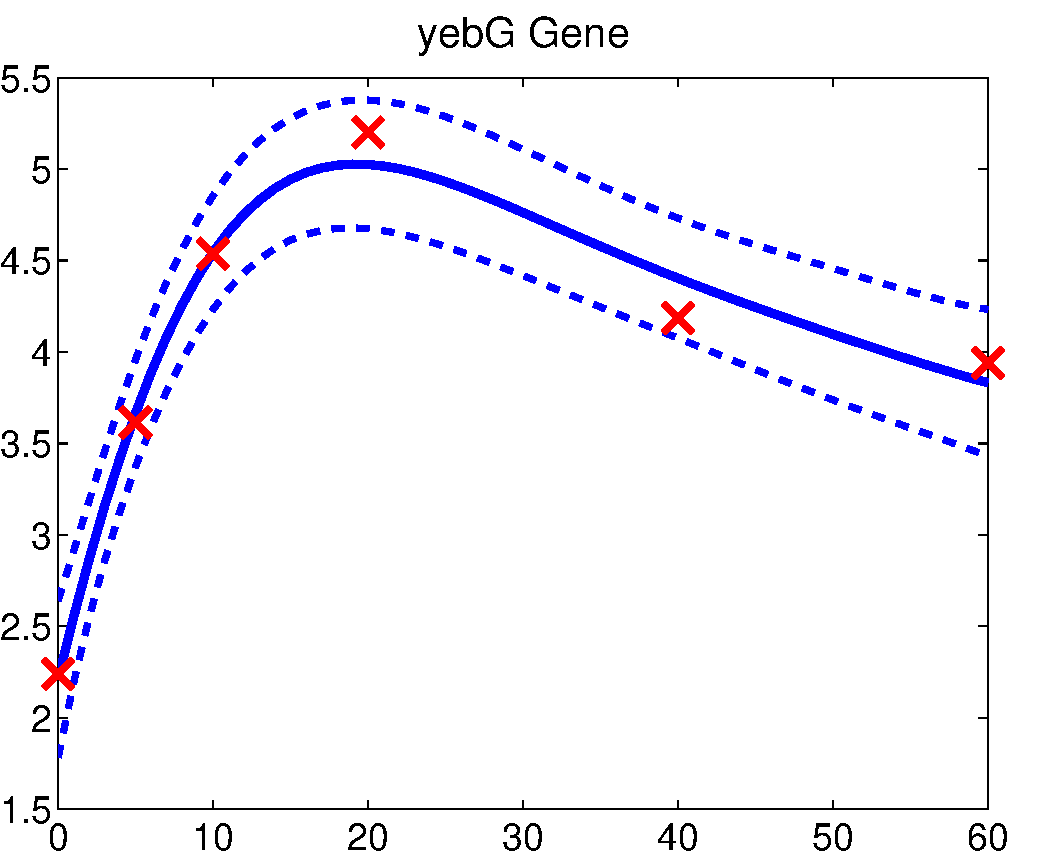
\includegraphics[width=35mm,height=33mm]
{demEcoliNoMCMC4RbfexpMichMentenRepres_ExprsProfile_Rep1_Gene13.pdf}&
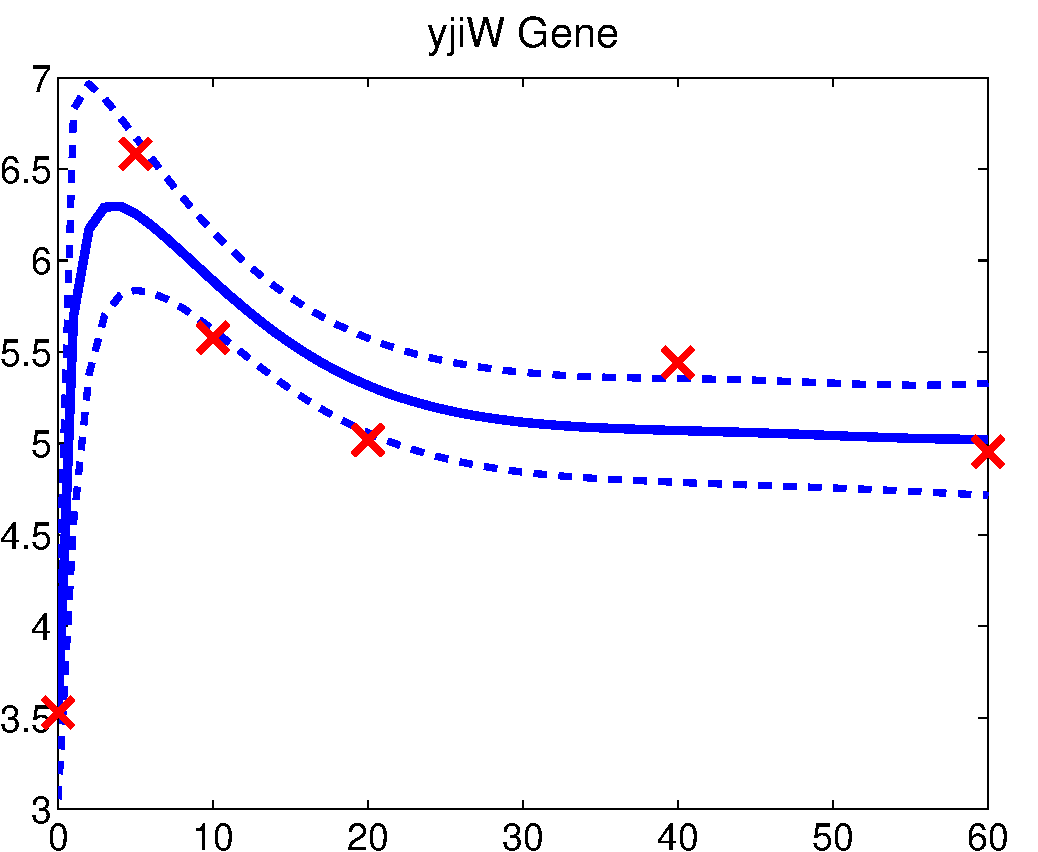
\includegraphics[width=35mm,height=33mm]
{demEcoliNoMCMC4RbfexpMichMentenRepres_ExprsProfile_Rep1_Gene14.pdf}
\end{tabular}
\end{center}
\end{figure}


}

\frame
{
 

\frametitle{Results in E.coli data: Protein concentration}


\begin{figure}
\begin{center}
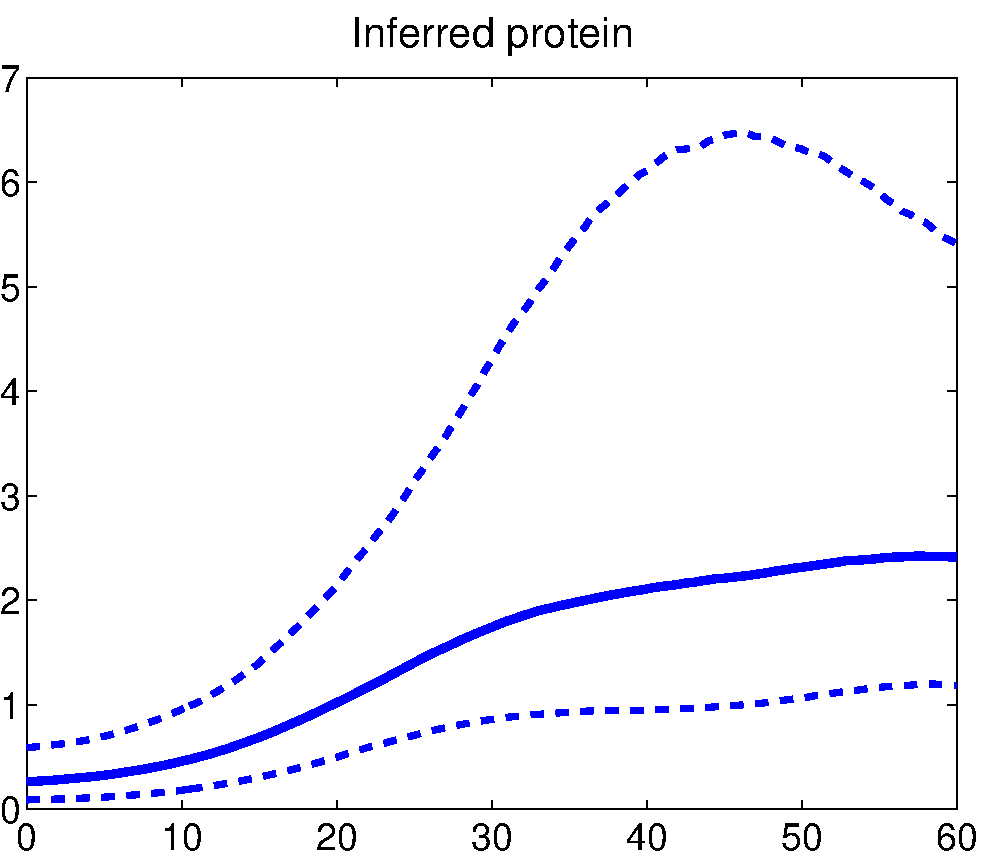
\includegraphics[width=90mm,height=70mm]
{demEcoliNoMCMC4RbfexpMichMentenRepres_profile1_slide.pdf}
\end{center}
\end{figure}


}

\frame
{

\frametitle{Results in E.coli data: Kinetic  parameters}


\begin{figure}
\begin{center}
\begin{tabular}{cc}
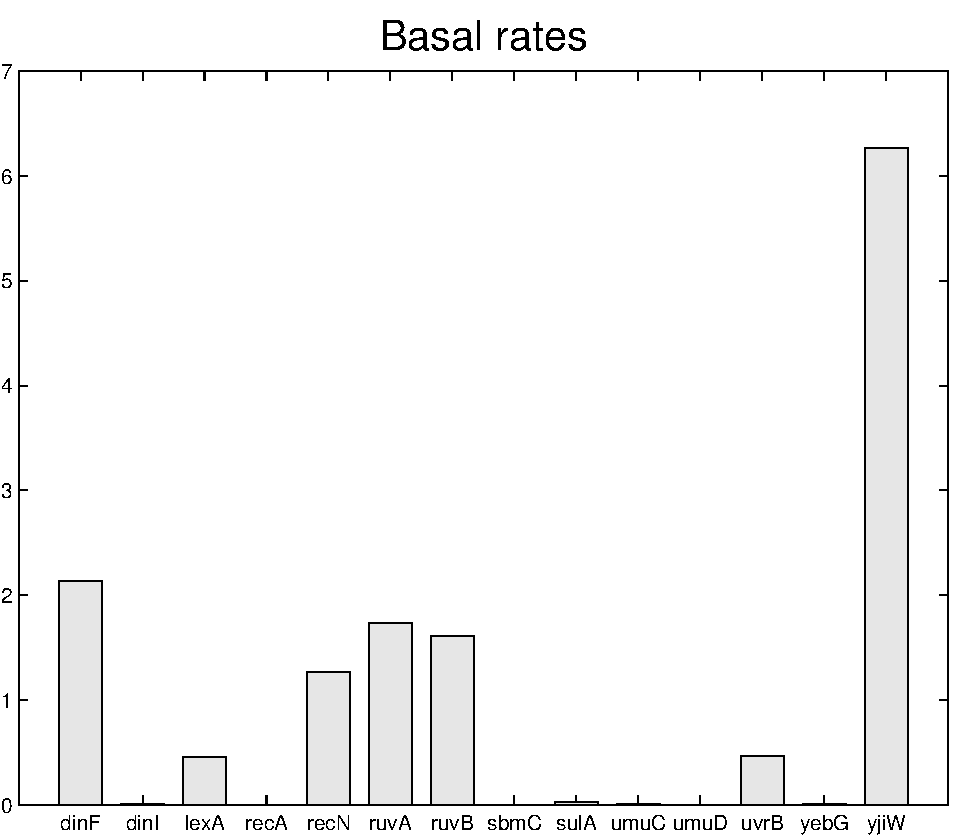
\includegraphics[width=48mm,height=31mm]
{demEcoliNoMCMC4RbfexpMichMentenRepres_basal.pdf}&
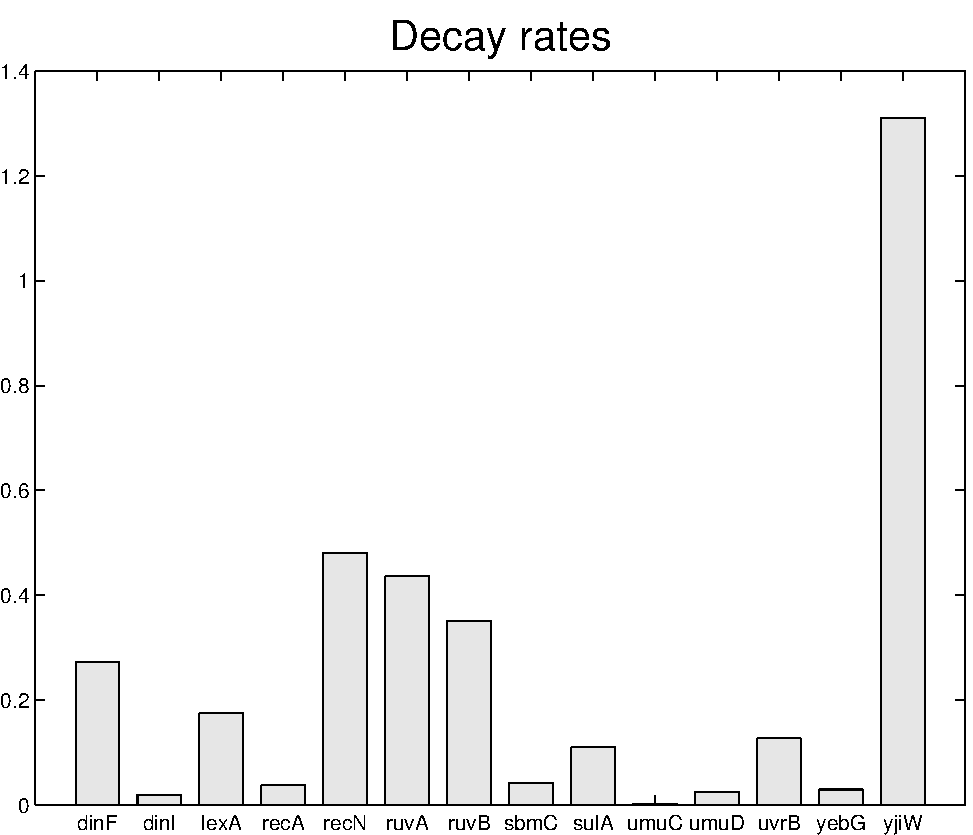
\includegraphics[width=48mm,height=31mm]
{demEcoliNoMCMC4RbfexpMichMentenRepres_decay.pdf} \\
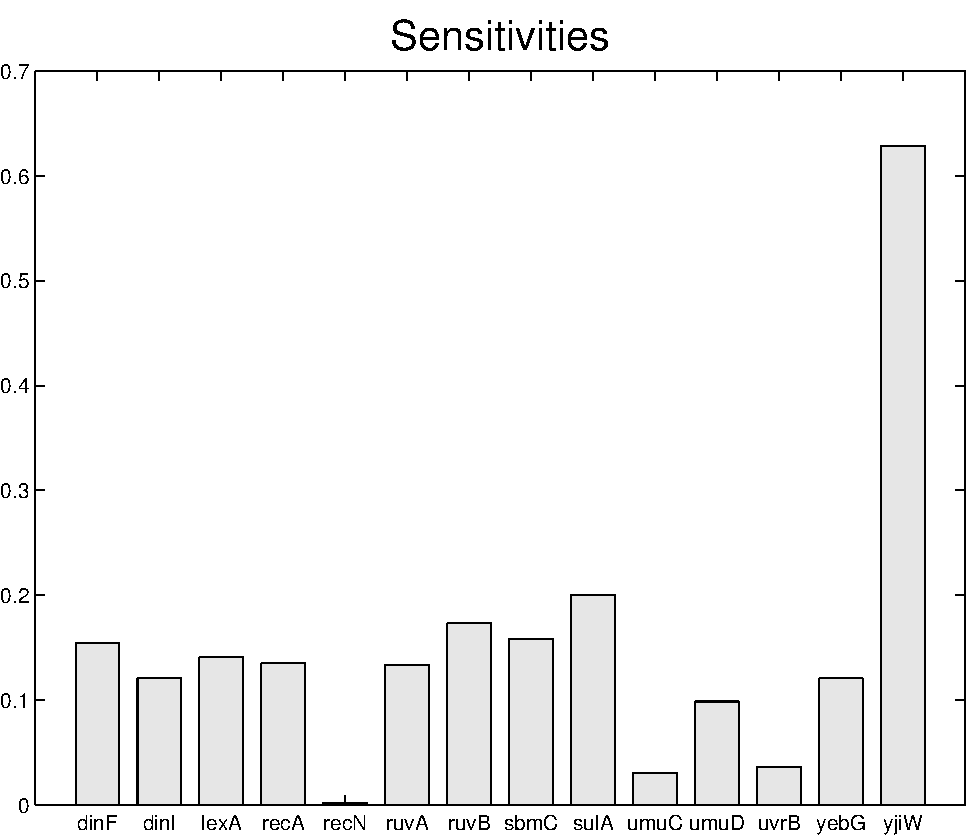
\includegraphics[width=48mm,height=31mm]
{demEcoliNoMCMC4RbfexpMichMentenRepres_sensitivity.pdf}&
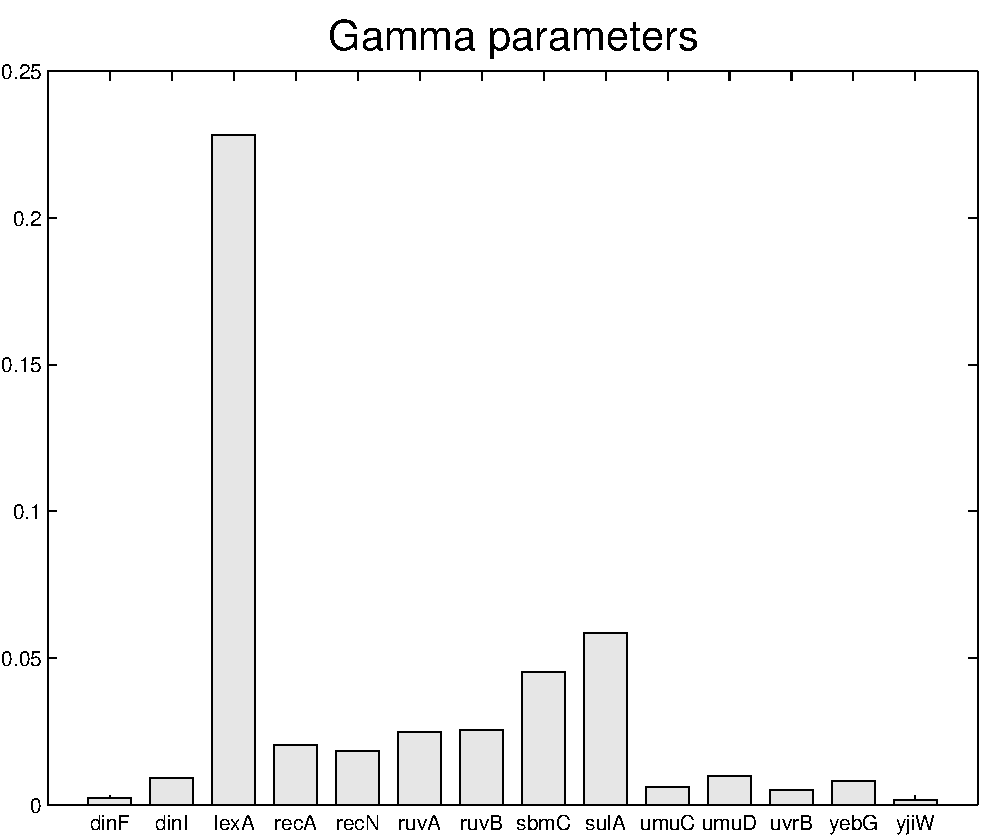
\includegraphics[width=48mm,height=31mm]
{demEcoliNoMCMC4RbfexpMichMentenRepres_gamma.pdf}
\end{tabular}
\end{center}
\end{figure}


}

\frame
{

\frametitle{Results in E.coli data: Genes with low sensitivity value}

\begin{figure}
\begin{center}
\begin{tabular}{ccc}
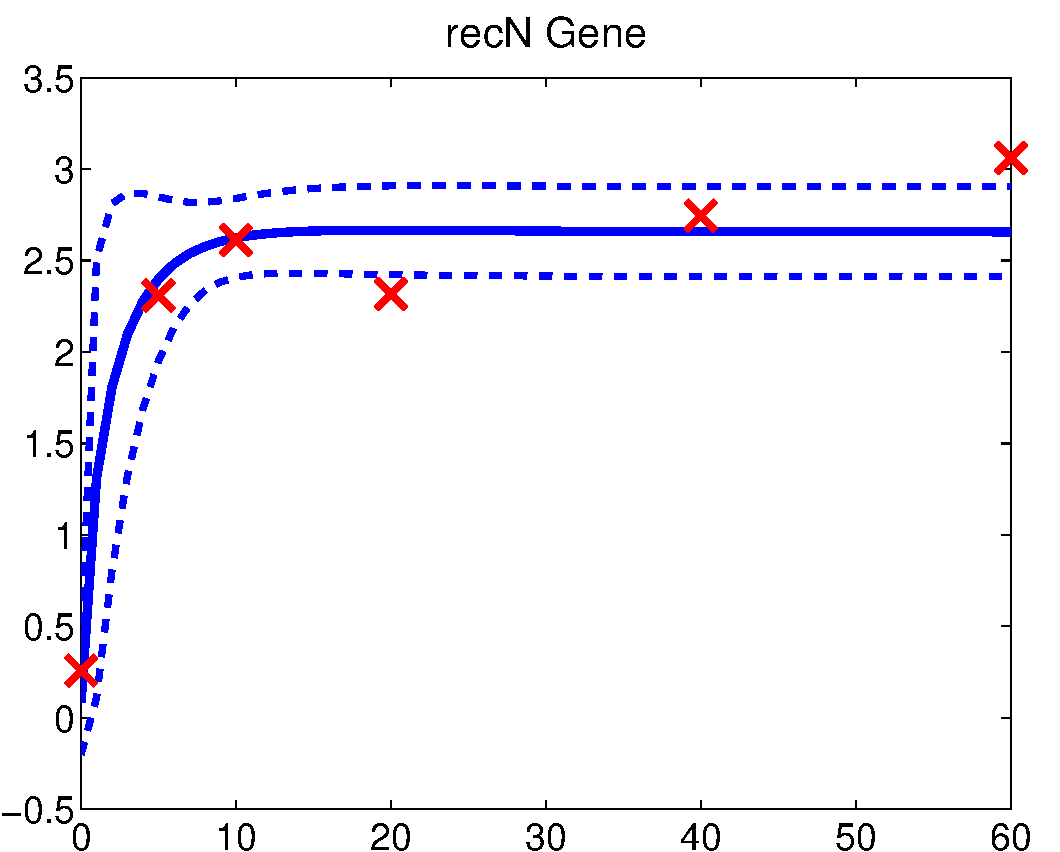
\includegraphics[width=34mm,height=31mm]
{demEcoliNoMCMC4RbfexpMichMentenRepres_ExprsProfile_Rep1_Gene5.pdf}&
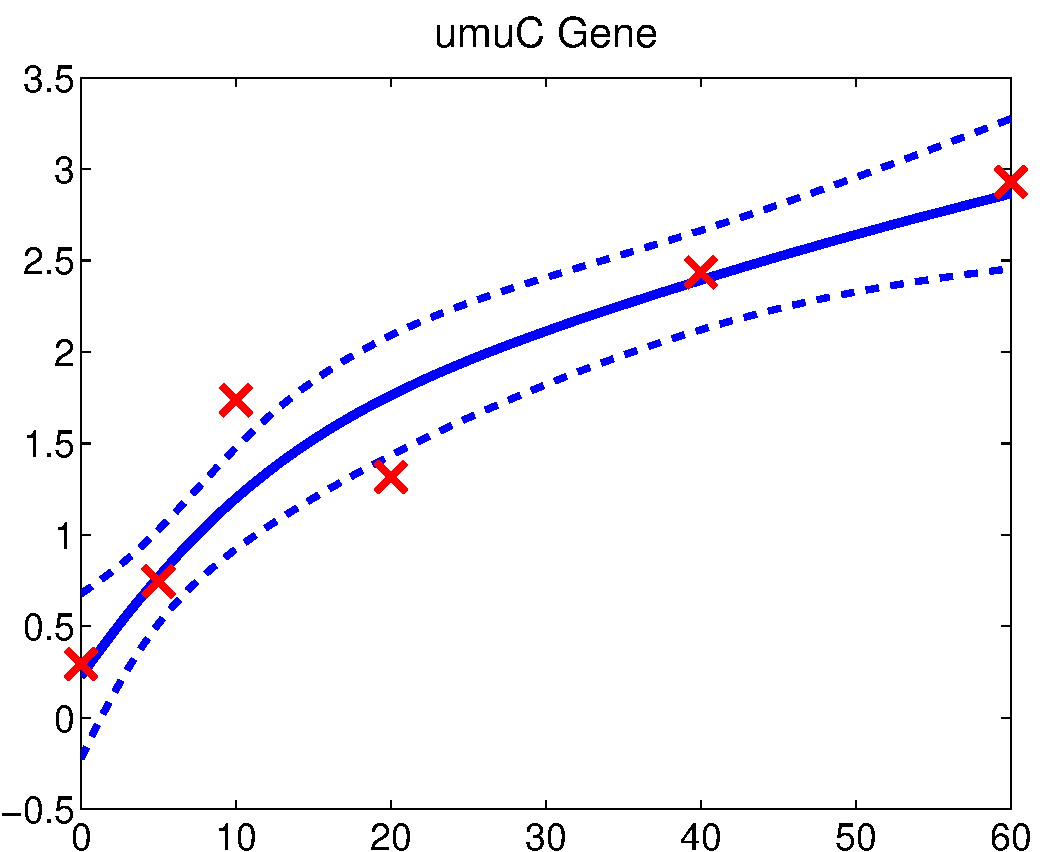
\includegraphics[width=34mm,height=31mm]
{demEcoliNoMCMC4RbfexpMichMentenRepres_ExprsProfile_Rep1_Gene10.pdf}&
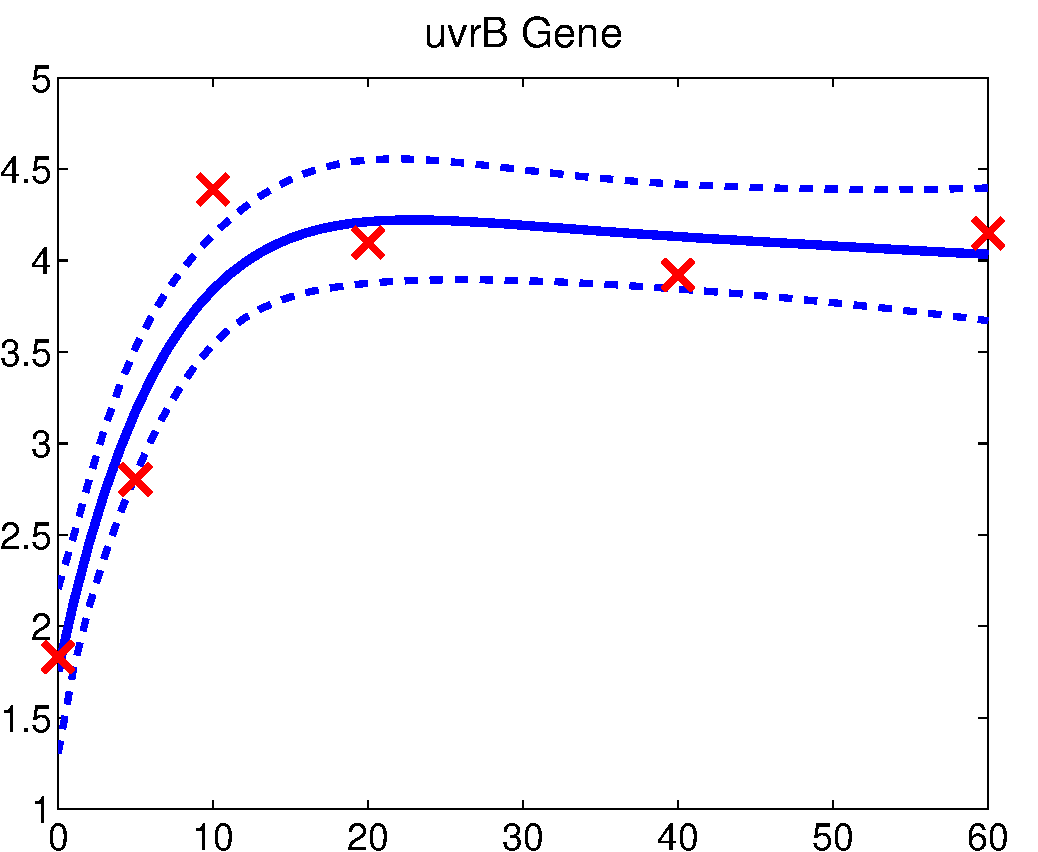
\includegraphics[width=34mm,height=31mm]
{demEcoliNoMCMC4RbfexpMichMentenRepres_ExprsProfile_Rep1_Gene12.pdf}
\end{tabular}
\end{center}
\end{figure}


\begin{figure}
\begin{center}
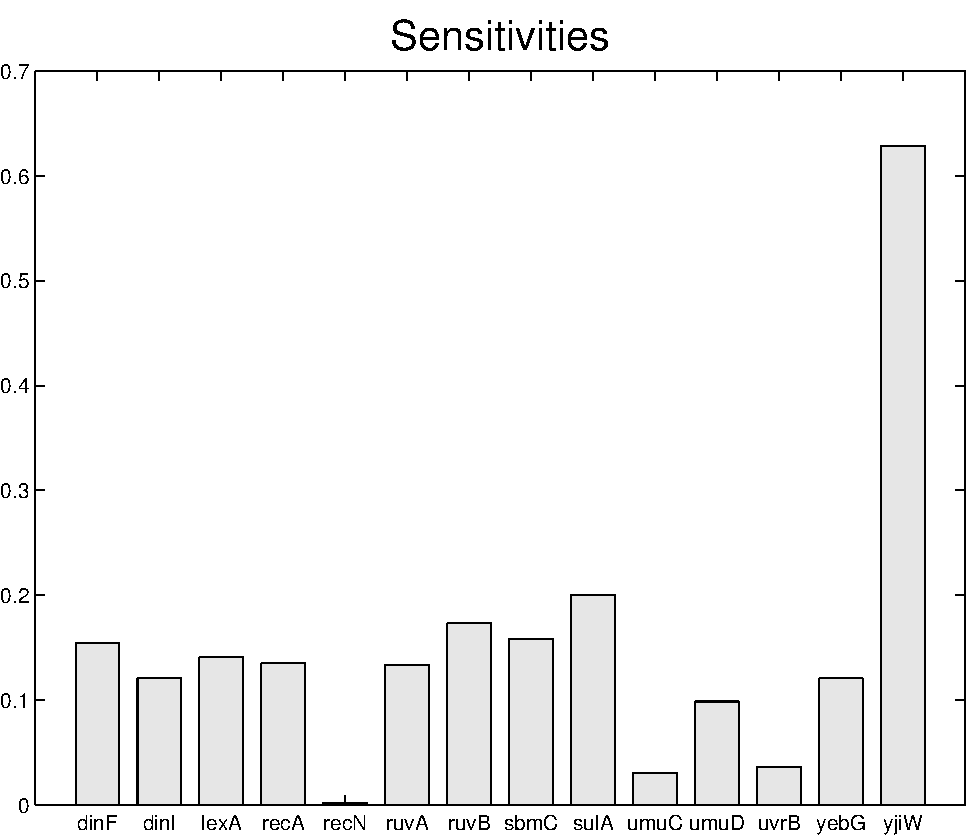
\includegraphics[width=65mm,height=38mm]
{demEcoliNoMCMC4RbfexpMichMentenRepres_sensitivity.pdf}
\end{center}
\end{figure}


}


\frame
{

\frametitle{Results in E.coli data: Confidence intervals for the
  kinetic parameters}


\begin{figure}
\begin{center}
\begin{tabular}{cc}
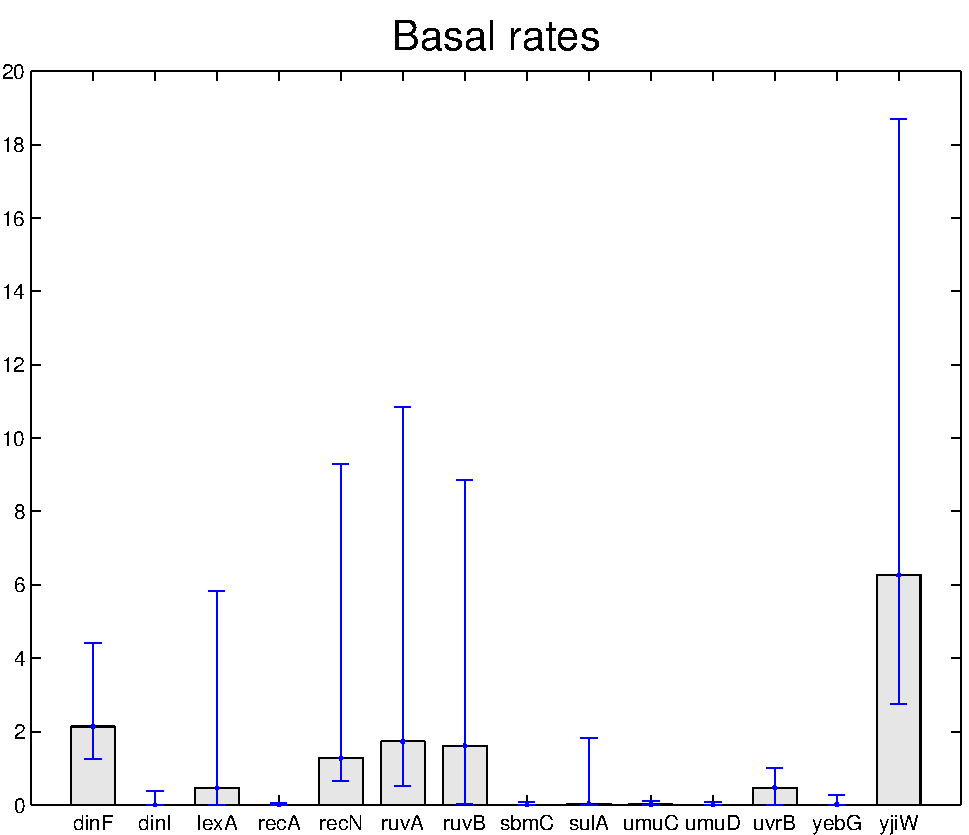
\includegraphics[width=48mm,height=31mm]
{demEcoliWithErrBarsNoMCMC4RbfexpMichMentenRepres_basal.pdf}&
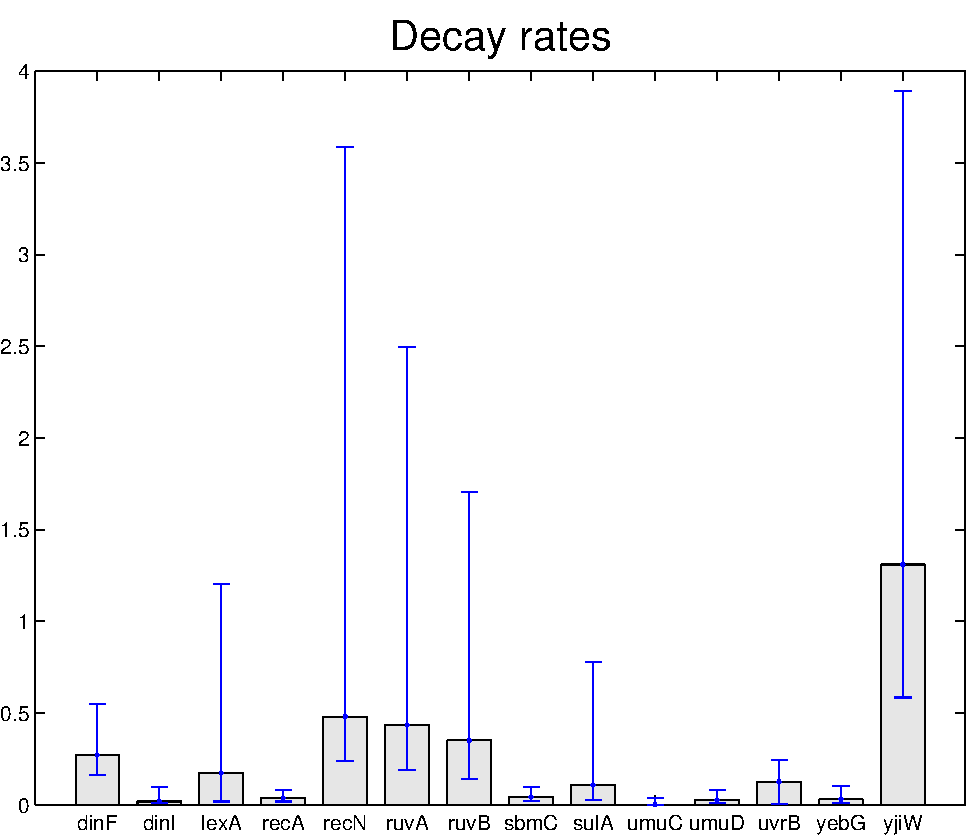
\includegraphics[width=48mm,height=31mm]
{demEcoliWithErrBarsNoMCMC4RbfexpMichMentenRepres_decay.pdf} \\
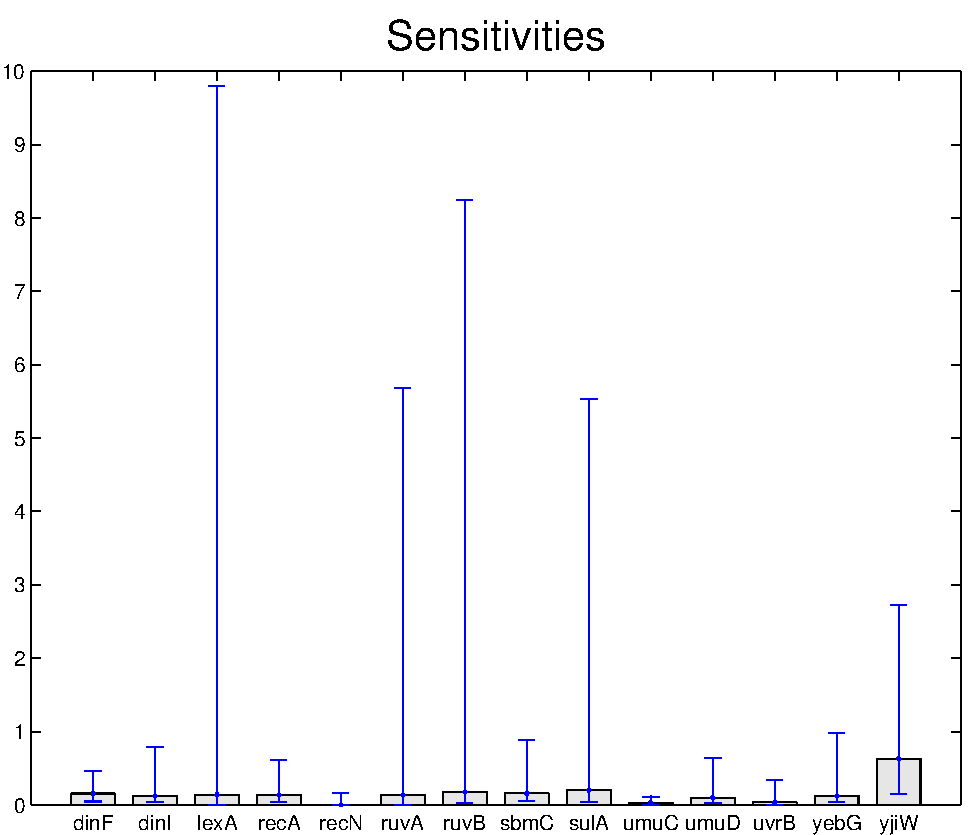
\includegraphics[width=48mm,height=31mm]
{demEcoliWithErrBarsNoMCMC4RbfexpMichMentenRepres_sensitivity.pdf}&
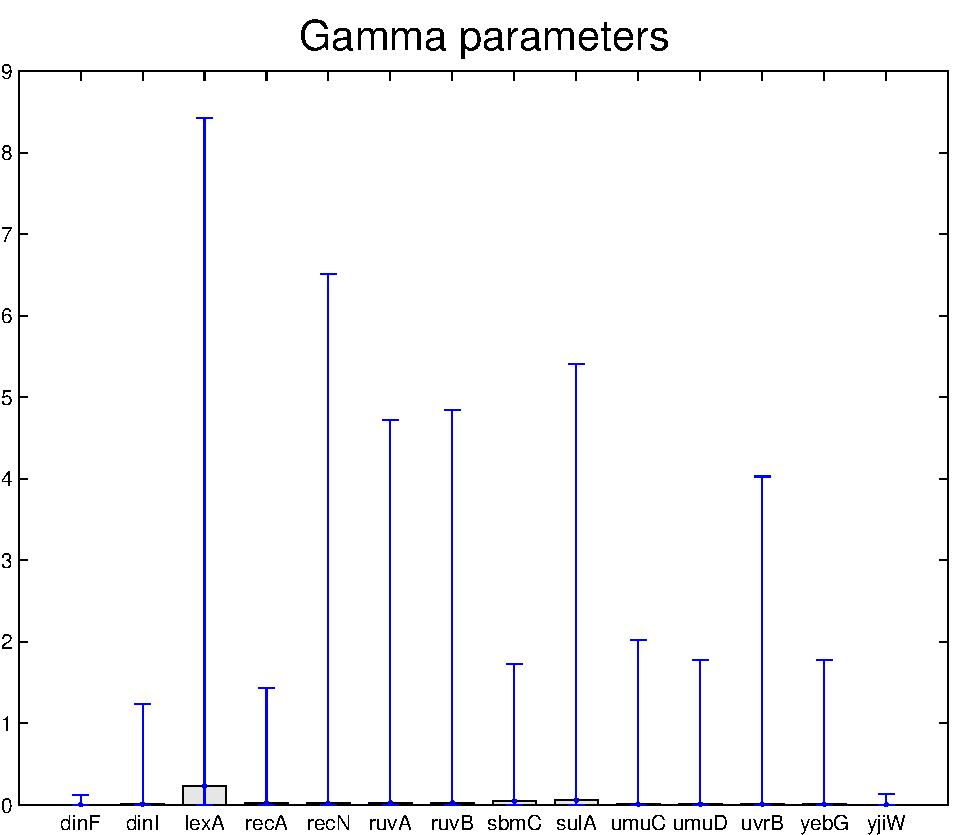
\includegraphics[width=48mm,height=31mm]
{demEcoliWithErrBarsNoMCMC4RbfexpMichMentenRepres_gamma.pdf}
\end{tabular}
\end{center}
\end{figure}

}

\frame
{
 

\frametitle{Data used by Barenco et al. [2006]}

\begin{itemize}
\item  One transcription factor (p53) that acts as an activator. We
  consider the Michaelis-Menten kinetic equation  
$$
\frac{d y_j (t)} {d t} =
B_j + S_j \frac{\exp(f(t))}{\exp(f(t)) + \gamma_j} - D_j y_j(t)
$$

\item We have 5 genes

\item Gene expressions are available for $T=7$ times and there are
      3 replicas of the time series data 

\item TF ($\bff$) is discretized using 121 points

\item MCMC details: 
\begin{itemize}
\item 7 control points are used (placed in a equally spaced grid)    
\item Running time 4/5 hours for 2 million sampling iterations plus
      burn in 
\item Acceptance rate for $\bff$ after burn in was between 
      $15\%-25\%$ 
\end{itemize}

\end{itemize}

}


\frame
{
 
\frametitle{Data used by Barenco et al. [2006]:  Predicted gene expressions for the
1st replica}


\begin{figure}
\begin{center}
\begin{tabular}{ccc}
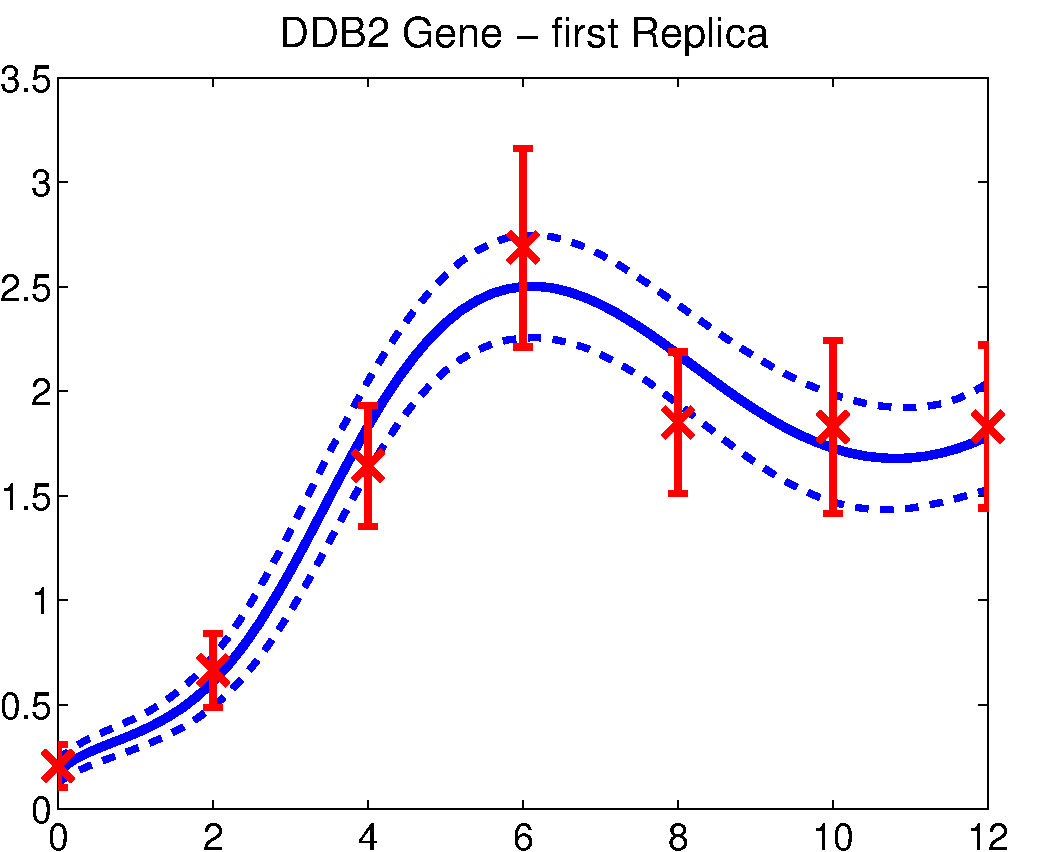
\includegraphics[width=35mm,height=33mm]
{demBarencoNoMCMC7RbfexpMichMentenAct_ExprsProfile_Rep1_Gene1.pdf}&
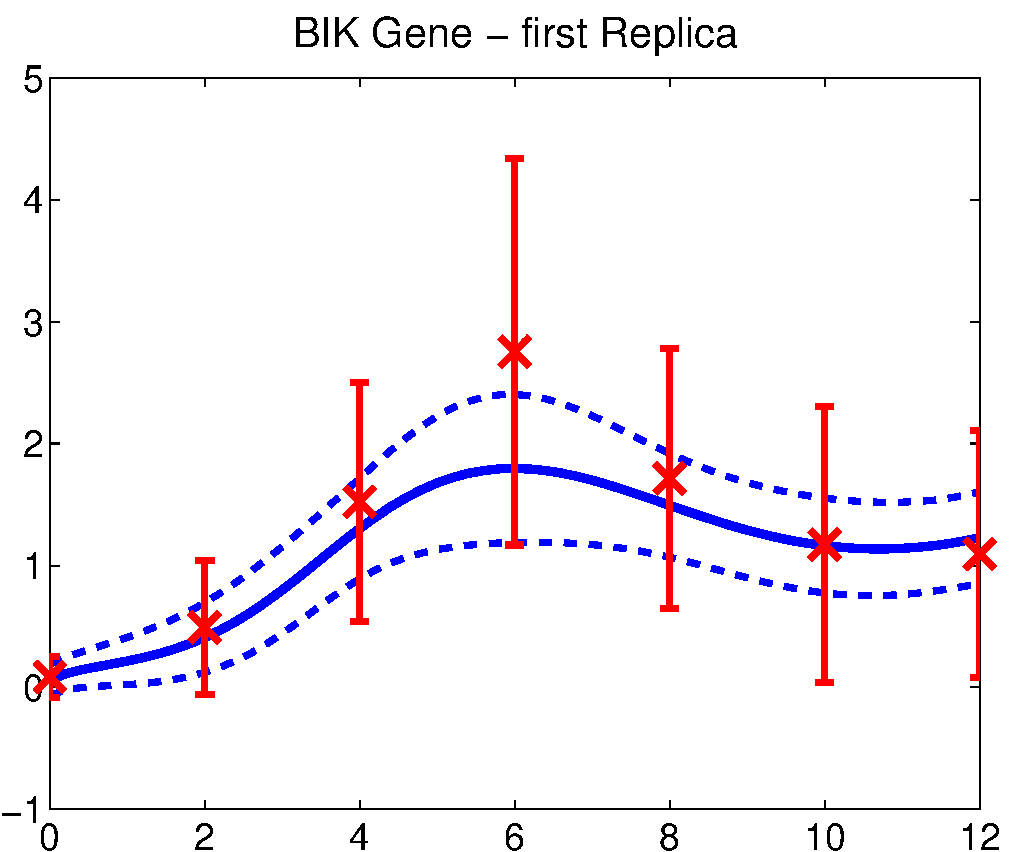
\includegraphics[width=35mm,height=33mm]
{demBarencoNoMCMC7RbfexpMichMentenAct_ExprsProfile_Rep1_Gene2.pdf}&
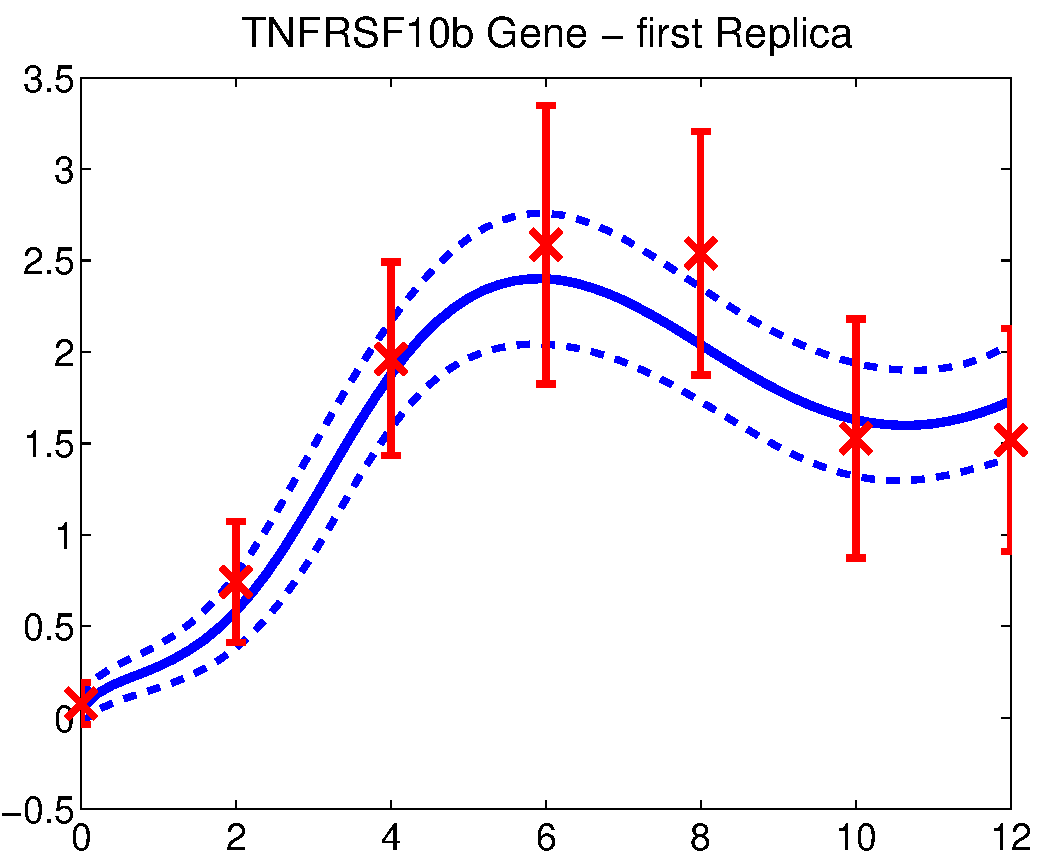
\includegraphics[width=35mm,height=33mm]
{demBarencoNoMCMC7RbfexpMichMentenAct_ExprsProfile_Rep1_Gene3.pdf} \\
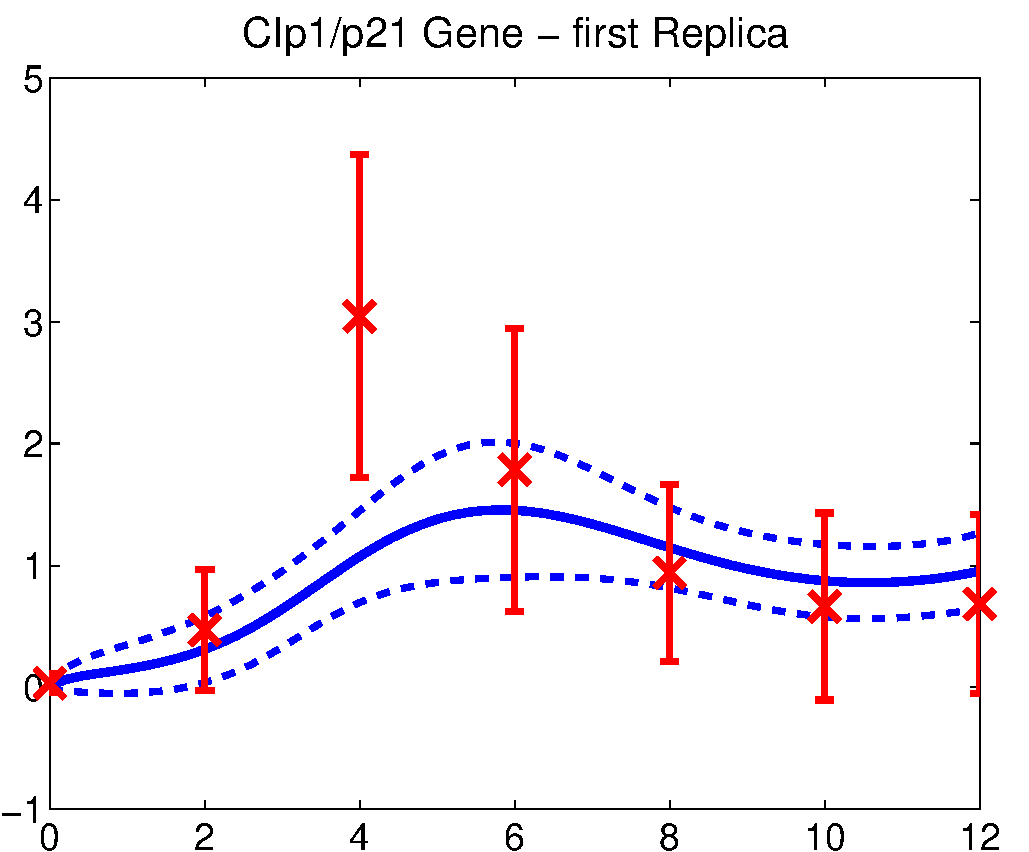
\includegraphics[width=35mm,height=33mm]
{demBarencoNoMCMC7RbfexpMichMentenAct_ExprsProfile_Rep1_Gene4.pdf}&
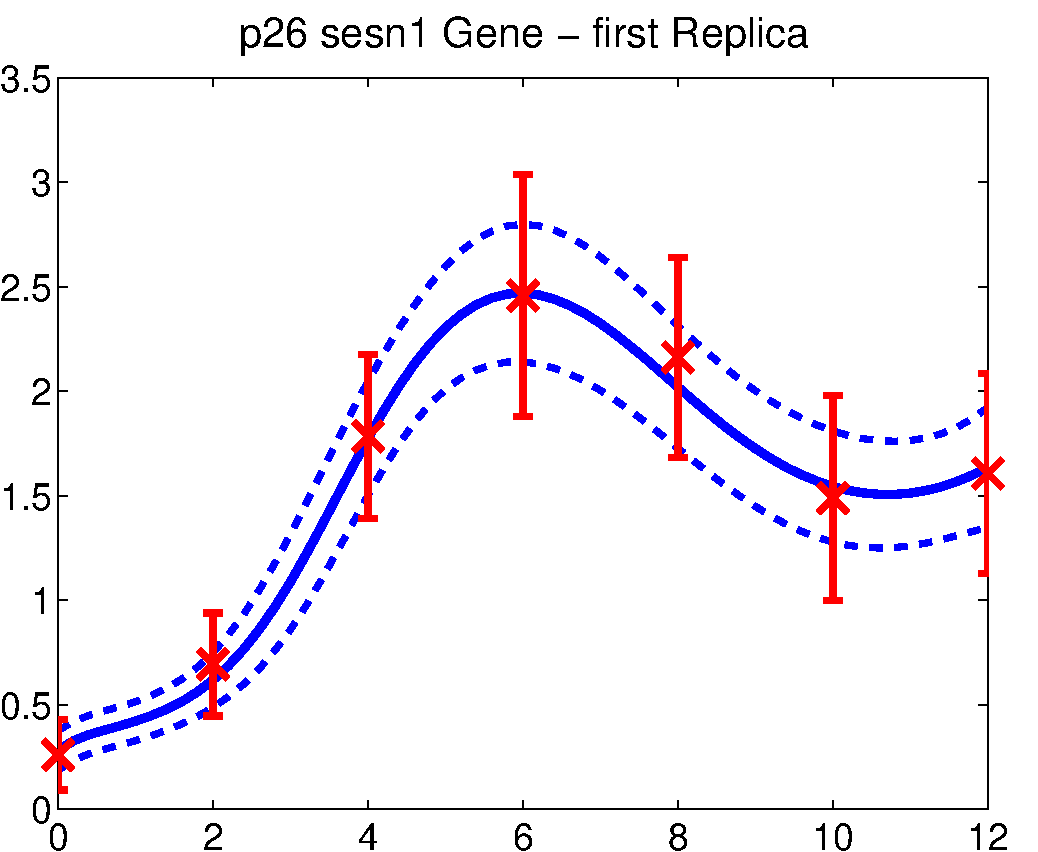
\includegraphics[width=35mm,height=33mm]
{demBarencoNoMCMC7RbfexpMichMentenAct_ExprsProfile_Rep1_Gene5.pdf}
\end{tabular}
\end{center}
\end{figure}


}


\frame
{
 
\frametitle{Data used by Barenco et al. [2006]: Protein concentrations}

\begin{figure}
\begin{center}
\begin{tabular}{ccc}
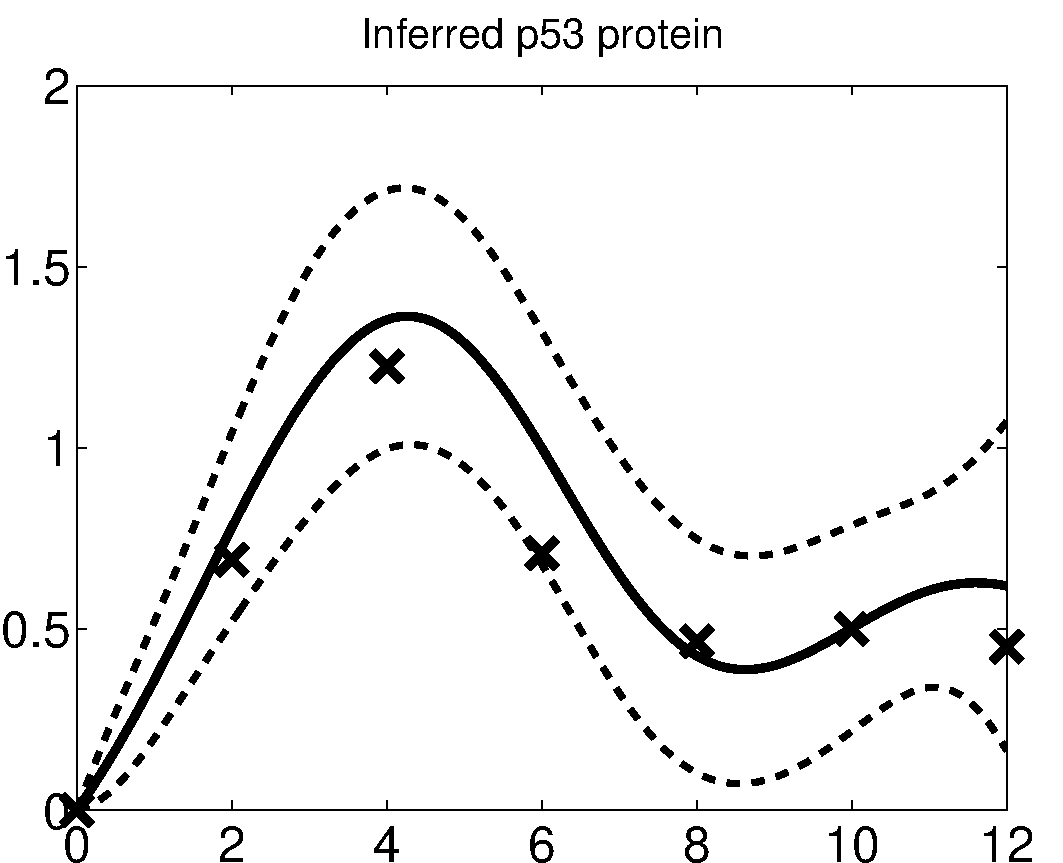
\includegraphics[width=35mm,height=26mm]
{demBarencoMCMC2Rbflinear_profile1_slide.pdf}&
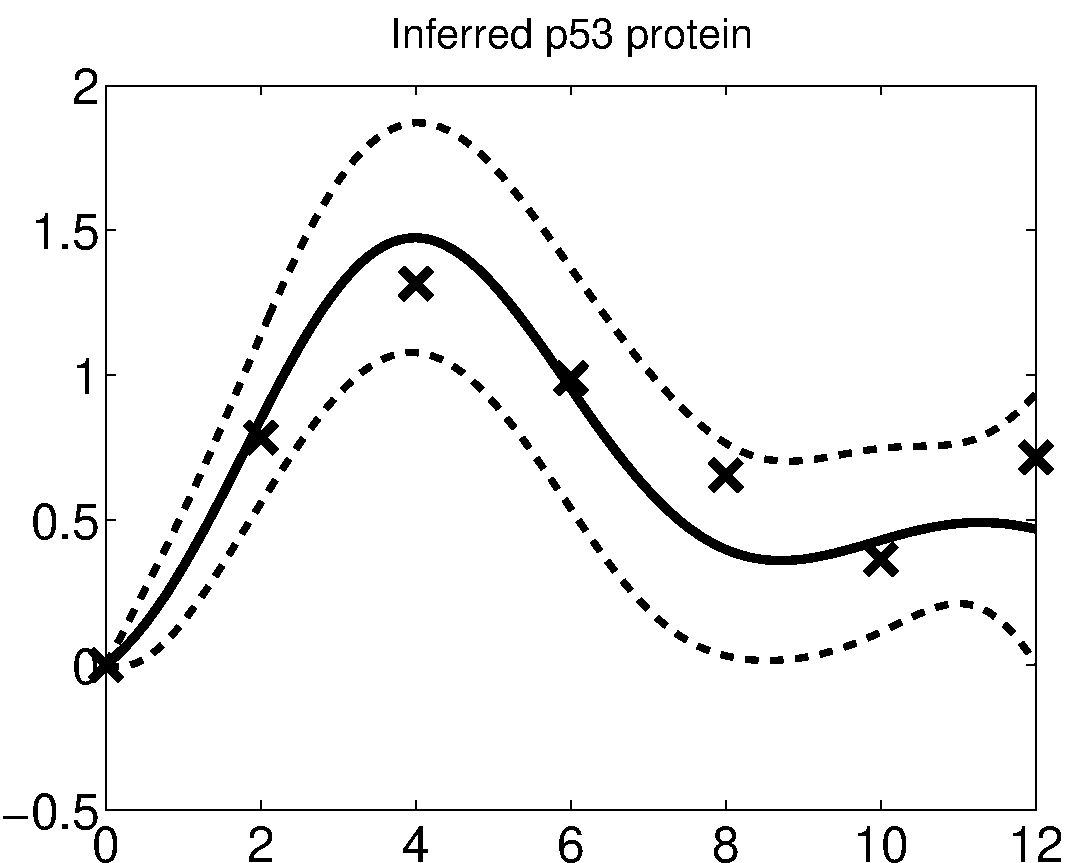
\includegraphics[width=35mm,height=26mm]
{demBarencoMCMC2Rbflinear_profile2_slide.pdf}&
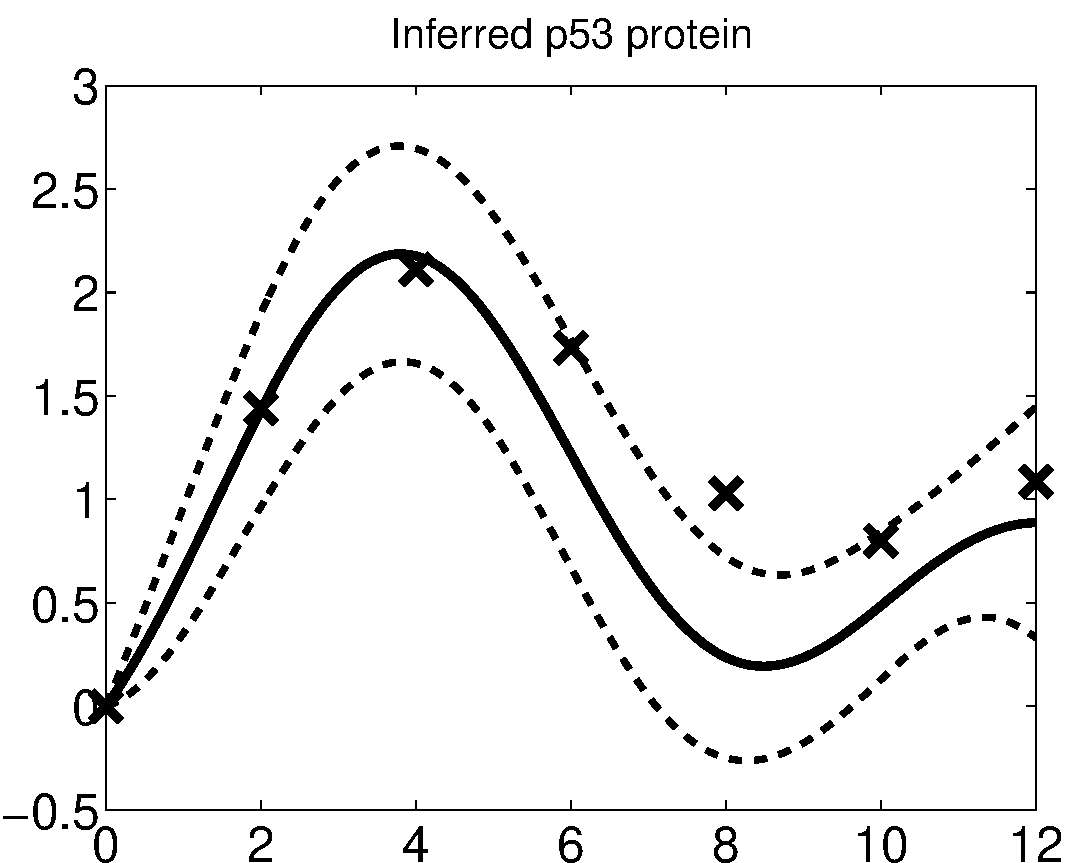
\includegraphics[width=35mm,height=26mm]
{demBarencoMCMC2Rbflinear_profile3_slide.pdf} 
\end{tabular}
\end{center}
\end{figure}
\centerline{Linear model (Barenco et al. predictions are shown as crosses)}
\begin{figure}
\begin{center}
\begin{tabular}{ccc}
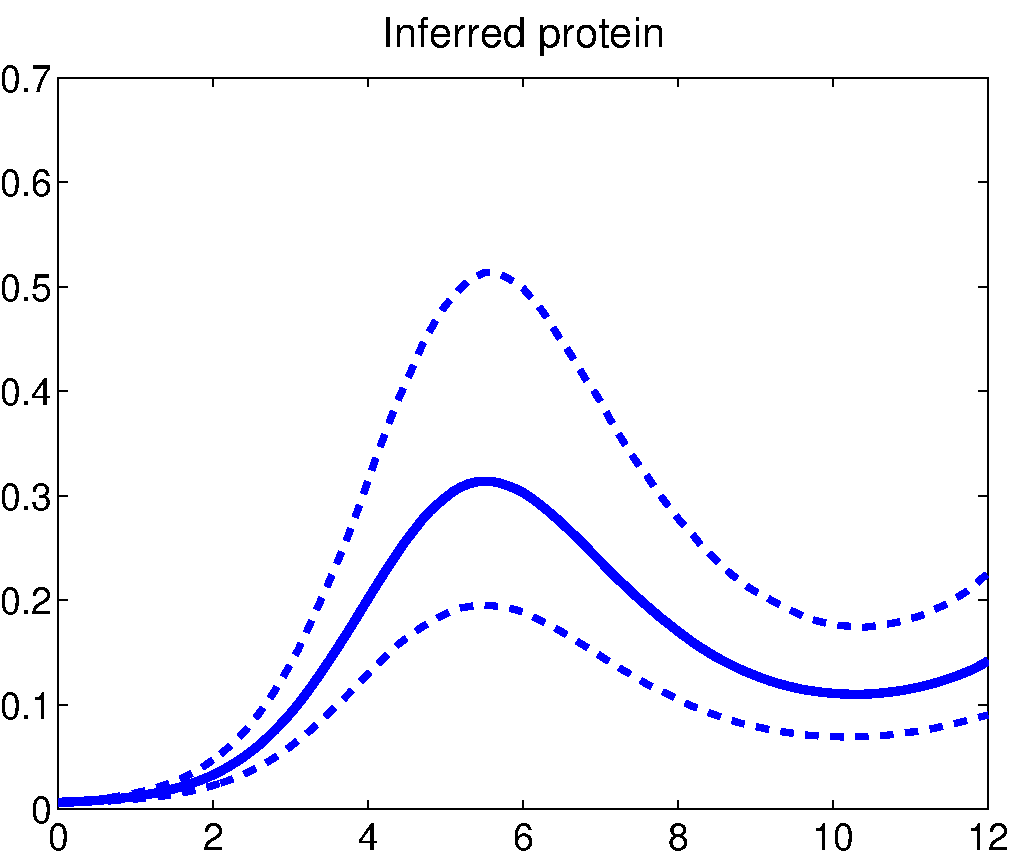
\includegraphics[width=35mm,height=26mm]
{demBarencoNoMCMC7RbfexpMichMentenAct_profile1_slide.pdf}&
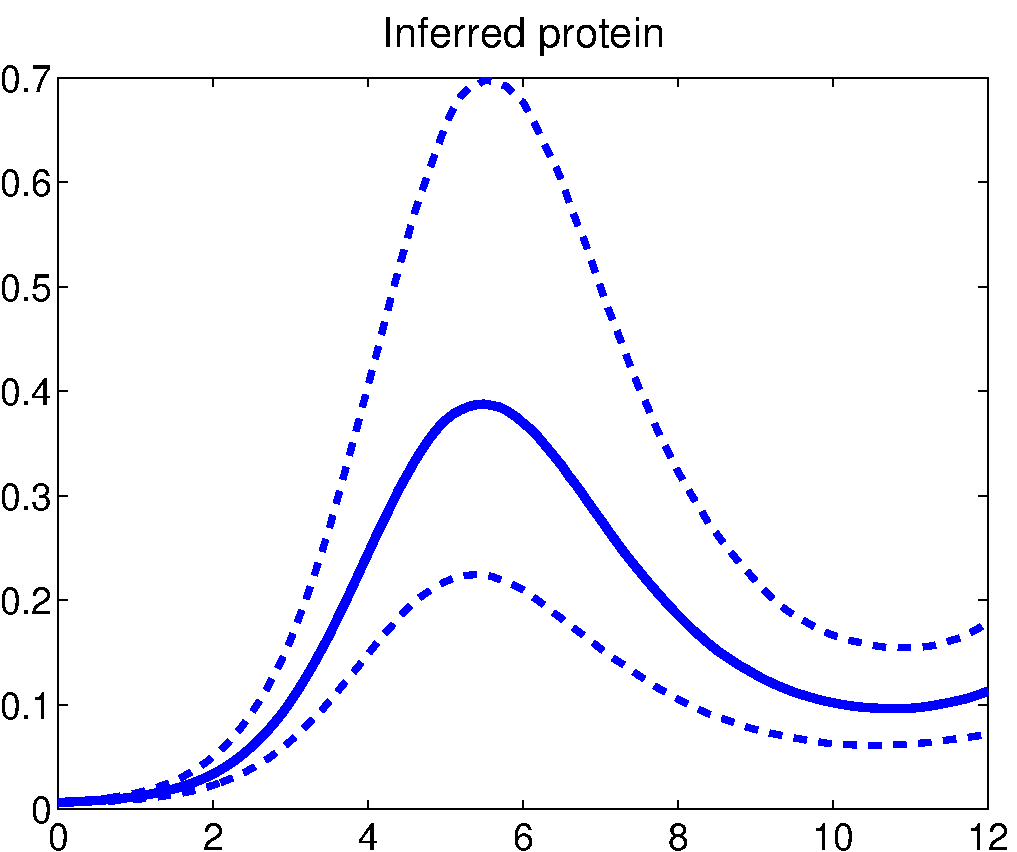
\includegraphics[width=35mm,height=26mm]
{demBarencoNoMCMC7RbfexpMichMentenAct_profile2_slide.pdf}&
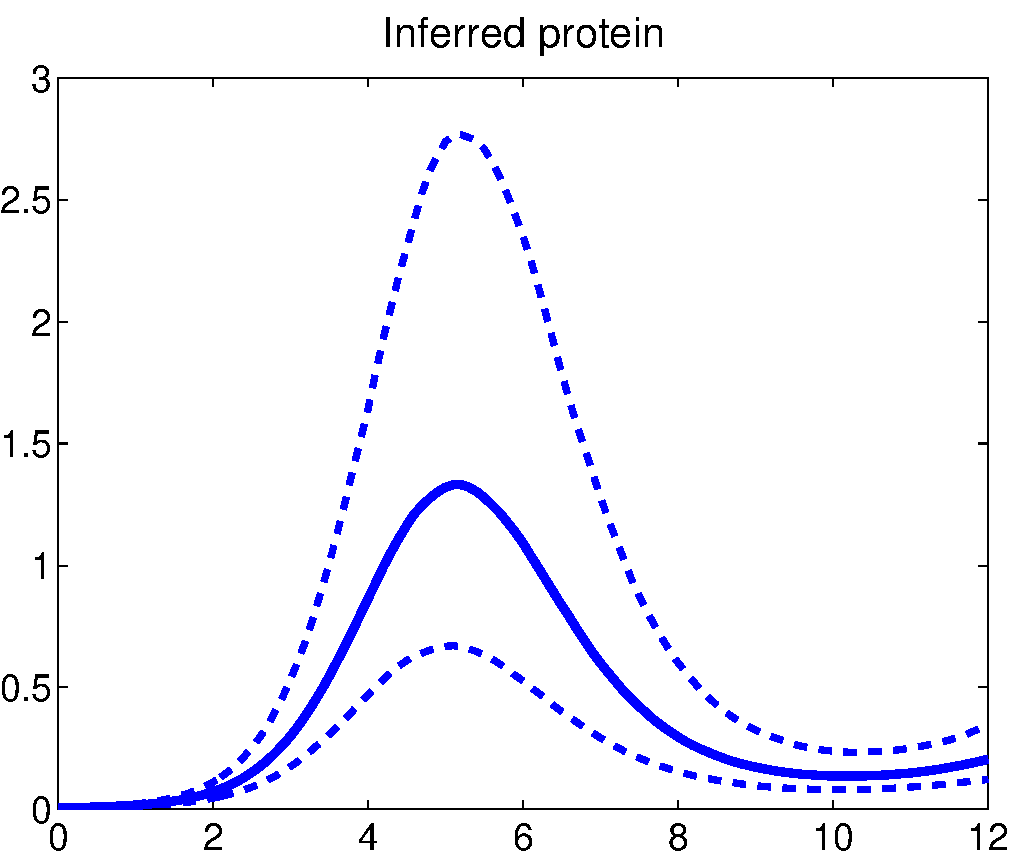
\includegraphics[width=35mm,height=26mm]
{demBarencoNoMCMC7RbfexpMichMentenAct_profile3_slide.pdf} 
\end{tabular}
\end{center}
\end{figure}
\centerline{Nonlinear (Michaelis-Menten kinetic equation)}
%\centerline{Protein concentration for the three replicas}

}


\frame
{
 
\frametitle{Data used by Barenco et al. [2006]: Kinetic parameters}



\begin{figure}
\begin{center}
\begin{tabular}{cc}
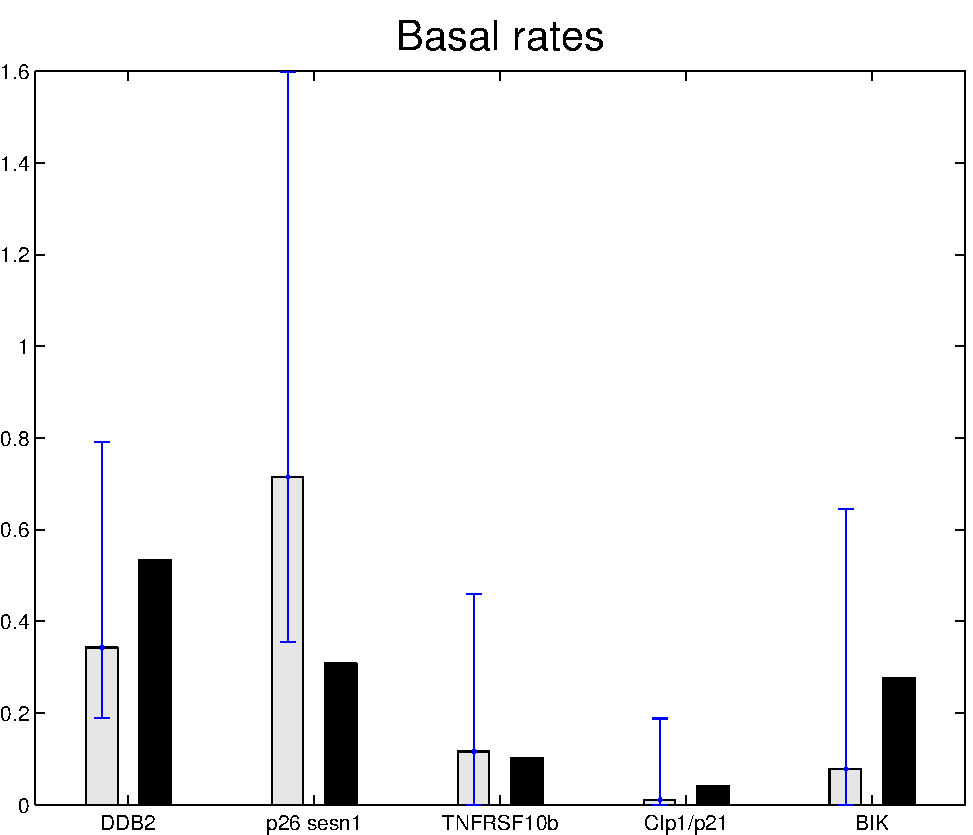
\includegraphics[width=45mm,height=31mm]
{demBarencoWithErrBarsNoMCMC7RbfexpMichMentenAct_basal.pdf}&
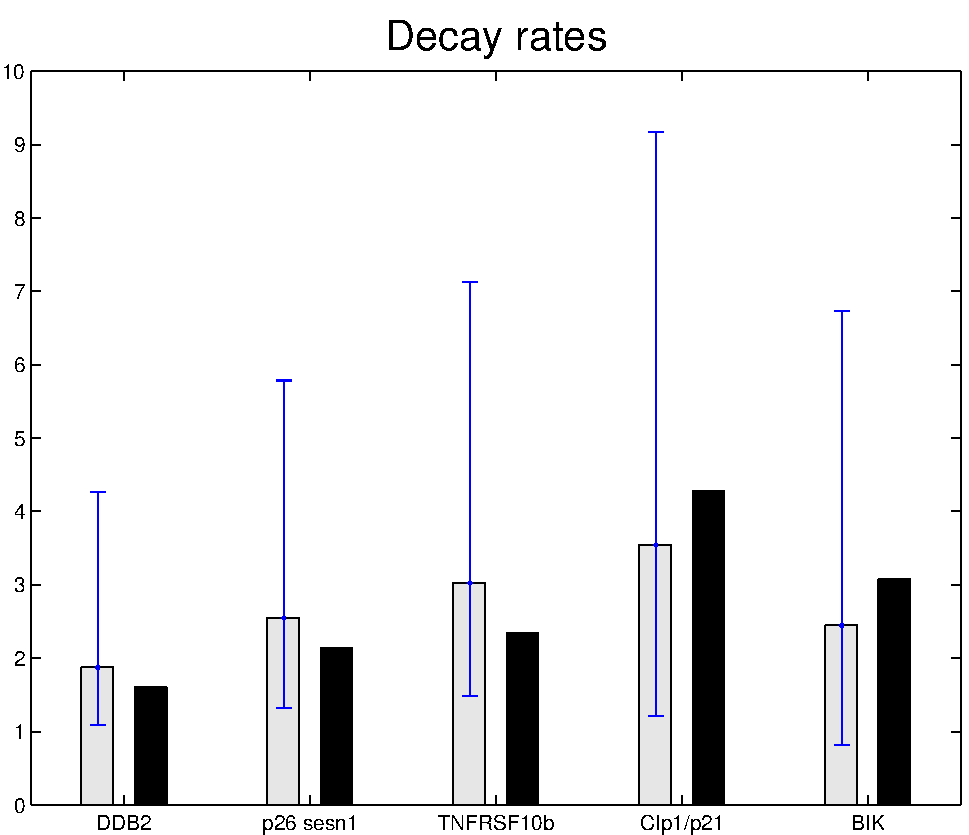
\includegraphics[width=45mm,height=31mm]
{demBarencoWithErrBarsNoMCMC7RbfexpMichMentenAct_decay.pdf} \\
\includegraphics[width=45mm,height=31mm]
{demBarencoWithErrBarsNoMCMC7RbfexpMichMentenAct_sensitivity.pdf}&
\includegraphics[width=45mm,height=31mm]
{demBarencoWithErrBarsNoMCMC7RbfexpMichMentenAct_gamma.pdf}
\end{tabular}
\end{center}
\end{figure}

Our results (grey) compared with Barenco et al. [2006]
  (black). Note that Barenco et al. use a linear model

}



\frame
{
 

\frametitle{Summary/Future work}


Summary:
\begin{itemize}

\item A new MCMC algorithm for Gaussian processes  using
  control points

\item Continuous full Bayesian inference in transcription factor 
      networks 


\end{itemize}


Future issues:
\begin{itemize}

\item Deal with larger systems of ODEs

\item Incorporate domain knowledge when you define priors over 
      parameters such as  the kinetic parameters

\end{itemize}


}




\end{document}